% ****************************************************************************************** % Dissertation template and document class for Princeton University
% Author  : Jeffrey Scott Dwoskin <jdwoskin@princeton.edu>
% Adapted from: http://www.math.princeton.edu/graduate/tex/puthesis.html
% ****************************************************************************************** %


%%% For print copies
%% set 'singlespace' option to set entire thesis to single space, and define "\printmode" to remove all hyperlinks for printed copies of the thesis. Delete all output files before changing this mode -- it will turn hyperref package on and off
%\documentclass[12pt,lot, lof, singlespace]{puthesis}
%\newcommand{\printmode}{}

%%% For the electronic copy, use doublespacing, define "\proquestmode" to use outlined links, instead of colored links. 
\documentclass[12pt,lot, lof]{puthesis}
\newcommand{\proquestmode}{}
%%% For early drafts without some of the frontmatter
% Also see the "ifodd" command below to disable more frontmatter
%\documentclass[12pt]{puthesis}
%\usepackage[letterpaper]{geometry}
\usepackage{titlesec}
\usepackage{booktabs}
\usepackage[superscript,biblabel]{cite}

%%%%%%%%%%%%%%%%%%%%%%%%%%%%%%%%%%%%%%%%%%%%%%%%%%%%%%%%%%%%%\
%%%% Author & title page info

\title{Gender differences in u.s. entrepreneurship decisions: an empirical analysis}

\submitted{April 5th, 2016}  % degree conferral date (January, April, June, September, or November)
\copyrightyear{2016}  % year in which the copyright is secured by publication of the dissertation.
\author{Roxana Carmen Turcanu}
\adviser{Roland Benabou}  %replace with the full name of your adviser
\departmentprefix{Faculty of the}  % defaults to "Department of", but programs need to change this.
\department{Woodrow Wilson School}

%%%%%%%%%%%%%%%%%%%%%%%%%%%%%%%%%%%%%%%%%%%%%%%%%%%%%%%%%%%%%\
%%%% Tweak float placements
% From: http://mintaka.sdsu.edu/GF/bibliog/latex/floats.html "Controlling LaTeX Floats"
% and based on: http://www.tex.ac.uk/cgi-bin/texfaq2html?label=floats
% LaTeX defaults listed at: http://people.cs.uu.nl/piet/floats/node1.html

% Alter some LaTeX defaults for better treatment of figures:
    % See p.105 of "TeX Unbound" for suggested values.
    % See pp. 199-200 of Lamport's "LaTeX" book for details.
    %   General parameters, for ALL pages:
    \renewcommand{\topfraction}{0.85}	% max fraction of floats at top
    \renewcommand{\bottomfraction}{0.6}	% max fraction of floats at bottom
    %   Parameters for TEXT pages (not float pages):
    \setcounter{topnumber}{2}
    \setcounter{bottomnumber}{2}
    \setcounter{totalnumber}{4}     % 2 may work better
    \setcounter{dbltopnumber}{2}    % for 2-column pages
    \renewcommand{\dbltopfraction}{0.66}	% fit big float above 2-col. text
    \renewcommand{\textfraction}{0.15}	% allow minimal text w. figs
    %   Parameters for FLOAT pages (not text pages):
    \renewcommand{\floatpagefraction}{0.66}	% require fuller float pages
	% N.B.: floatpagefraction MUST be less than topfraction !!
    \renewcommand{\dblfloatpagefraction}{0.66}	% require fuller float pages

% The documentclass already sets parameters to make a high penalty for widows and orphans. 

%%%%%%%%%%%%%%%%%%%%%%%%%%%%%%%%%%%%%%%%%%%%%%%%%%%%%%%%%%%%%\
%%%% Use packages

%\usepackage{amsfonts}

%%% For figures
\usepackage{graphicx}
%\usepackage{subfig,rotate}

%%% for comments
\usepackage{verbatim}

%%% For tables
\usepackage{multirow}
% Longtable lets you have tables that span multiple pages.
\usepackage{longtable}

%For equations
\usepackage{breqn}

% Booktabs produces far nicer tables than the standard LaTeX tables.
%   see: http://en.wikibooks.org/wiki/LaTeX/Tables
\usepackage{booktabs}

%set parameters for longtable:
% default caption width is 4in for longtable, but wider for normal tables
\setlength{\LTcapwidth}{\textwidth}



%%%%%%%%%%%%%%%%%%%%%%%%%%%%%%%%%%%%%%%%%%%%%%%%%%%%%%%%%%
%%% Printed vs. online formatting
\ifdefined\printmode

% Printed copy
% url package understands urls (with proper line-breaks) without hyperlinking them
\usepackage{url}


\else

\ifdefined\proquestmode
%ProQuest copy -- http://www.princeton.edu/~mudd/thesis/Submissionguide.pdf

% ProQuest requires a double spaced version (set previously). They will take an electronic copy, so we want links in the pdf, but also copies may be printed or made into microfilm in black and white, so we want outlined links instead of colored links.
\usepackage{hyperref}
\hypersetup{bookmarksnumbered}

% copy the already-set title and author to use in the pdf properties
\makeatletter
\hypersetup{pdftitle=\@title,pdfauthor=\@author}
\makeatother

\else
% Online copy

% adds internal linked references, pdf bookmarks, etc

% turn all references and citations into hyperlinks:
%  -- not for printed copies
% -- automatically includes url package
% options:
%   colorlinks makes links by coloring the text instead of putting a rectangle around the text.
\usepackage{hyperref}
\hypersetup{colorlinks,bookmarksnumbered}

% copy the already-set title and author to use in the pdf properties
\makeatletter
\hypersetup{pdftitle=\@title,pdfauthor=\@author}
\makeatother

% make the page number rather than the text be the link for ToC entries
%\hypersetup{linktocpage}
\fi % proquest or online formatting
\fi % printed or online formatting


%%%%%%%%%%%%%%%%%%%%%%%%%%%%%%%%%%%%%%%%%%%%%%%%%%%%%%%%%%%%%\
%%%% Define commands

% Define any custom commands that you want to use.
% For example, highlight notes for future edits to the thesis
%\newcommand{\todo}[1]{\textbf{\emph{TODO:}#1}}


% create an environment that will indent text
% see: http://latex.computersci.org/Reference/ListEnvironments
% 	\raggedright makes them left aligned instead of justified
\newenvironment{indenttext}{
    \begin{list}{}{ \itemsep 0in \itemindent 0in
    \labelsep 0in \labelwidth 0in
    \listparindent 0in
    \topsep 0in \partopsep 0in \parskip 0in \parsep 0in
    \leftmargin 1em \rightmargin 0in
    \raggedright
    }
    \item
  }
  {\end{list}}

% another environment that's an indented list, with no spaces between items -- if we want multiple items/lines. Useful in tables. Use \item inside the environment.
% 	\raggedright makes them left aligned instead of justified
\newenvironment{indentlist}{
    \begin{list}{}{ \itemsep 0in \itemindent 0in
    \labelsep 0in \labelwidth 0in
    \listparindent 0in
    \topsep 0in \partopsep 0in \parskip 0in \parsep 0in
    \leftmargin 1em \rightmargin 0in
    \raggedright
    }

  }
  {\end{list}}



%%%%%%%%%%%%%%%%%%%%%%%%%%%%%%%%%%%%%%%%%%%%%%%%%%%%%%%%%%%%%\
%%%% Front-matter

\ifodd 0
\renewcommand{\maketitlepage}{}
\renewcommand*{\makecopyrightpage}{}
\renewcommand*{\makeabstract}{}

\else

\dedication{To my mother,\\
who made all of it possible.}

\acknowledgements{
%I would like to thank...
I would like to thank 

My adviser, for guiding me through this daunting process. \par

My family, for loving me more than anything. You were, and will always be, my home and my anchor through it all. \par

Ioana, for always being the magical intervention in my life. I love and admire your spirit, and I would poster with you anytime, anywhere. \par

Izzy, for being my unconditional friend, my little piece of Rio and one of the most beautifully inspiring human beings I know. \par

Cezar, for being my Pushnik, my spontaneity and my spoiled, . I'm lucky to have jumped from that airplane with you. \par

Terrace F. Club, because it exists.\par

All the loose ends that made me who I am today.


}

\abstract{
\singlespacing 

The current paper models the determinants of entrepreneurship entry decisions at the U.S. level, asking whether and how men and women respond differently to factors of interest. The probability of someone becoming an entrepreneur is estimated via a Probit Model, as a function of socio-economic factors, demographic controls, local business climate, liquidity constraints and occupational choice. For every model, errors are clustered by metropolitan area, and coefficient equality is tested across gender samples. At the individual level, we find that availability of capital remains an important factor, along with skill versatility, education and minority status. When it comes to external factors, we find women are incentivized to a greater extent by tax credits and the state of the political climate, while men respond to positive changes in the local economy. Across industries, we find patterns of women being underrepresented in STEM fields, which is consistent with the case of wage employment and disproves our hypothesis of a breaking-barriers mechanism to starting one's business. 

\singlespacing \textbf{Keywords:} gender, entrepreneurship, self-employment, innovation, economic growth, incentives, asymmetry, female labor force participation.

\bodyspacing
}

\fi  % disable frontmatter

%%%%%%%%%%%%%%%%%%%%%%%%%%%%%%%%%%%%%%%%%%%%%%%%%%%%%%%%%%%%%
%%%% Notes:

% Footnotes should be placed after punctuation.\footnote{place here.}
% Generally, place citations before the period~\cite{anotherauthor}.
% The proper usage for i.e., and e.g., include commas ``(e.g., option A, option B)''

%%%% Chapter title styling:
\titleformat{\chapter}[display]
  {\normalfont\bfseries}{}{0pt}{\huge}
\titlespacing*{\chapter}{0pt}{*1}{*5}

%%%%%%%%%%%%%%%%%%%%%%%%%%%%%%%%%%%%%%%%%%%%%%%%%%%%%%%%%%%%%
%%%% Import chapters

\begin{document}

\makefrontmatter

% \include lets us split up the document (and each include starts a new page):
\chapter{Introduction\label{ch:intro}}

\begin{flushright}
    \textit{"For many commentators this is the era of the entrepreneur." } \\
    (Robert Goffee and Richard Scase)
\end{flushright}


Entrepreneurship: it has become an almost commonplace preoccupation in American society, treated with great interest by both the general public, and specialized literature---with more and more consensus regarding its beneficial impact for employment, innovation and growth for the economy at large\footnote{\cite{ReynoldsWhite1997}}. With more than 10\% of the U.S. population working for their own company at a given time\footnote{Authors \cite{bucks2006recent} invoke this makes for 13 million business owners holding an astounding 37.4\% percent of total U.S. wealth. }, and another large proportion indicating they would want to pursue this path\footnote{\cite{kennickell2006currents}}, it is without doubt a topic worthy of increased attention from policy makers. Nonetheless, the calls for policy action to expand on U.S. entrepreneurial activity via investment, research and development, or educational programs are frequently substantiated by an incomplete understanding of the process of  firm creation.  The focus is often on the new entity and its subsequent success, with little consideration for the individual agent as the major driver of economic value in a new organization\footnote{\cite{BlanchflowerOswald1998}}. But isn't that one of the main appeals, and promises of entrepreneurship---that of creativity and independence, of empowering individuals?

When the individual level is considered, one of the most significant differences pertaining to
entrepreneurship is noted in the proportion of men and women who choose to pursue business formation. Studies bluntly conclude that women are less likely to start their own business\footnote{\cite{kennickell2006currents}}\hspace{.15em}\footnote{\cite{PatrickStephensWeinstein2016}}\hspace{.15em}\footnote{\cite{koellinger2013gender}}, or less likely to apply for business loans\footnote{\cite{SBA}}, this in turn leading to profound implications for aggregate productivity, regional growth and gender parity in the labor market\footnote{\cite{ReynoldsWhite1997}}. Yet women's share of both self-employment and overall employment is on a continuous rise\footnote{\cite{PatrickStephensWeinstein2016}}, making the study of the factors affecting these decisions particularly important to our understanding of the U.S. labor force and its economic prospects. As increases in entrepreneurship and self-employment have been proven to be closely followed by economic growth\footnote{\cite{ReynoldsWhite1997}}, it is especially important to capture what incentivizes women to become self-employed and let such insights make for policy that caters to the economic agent, and not just the enterprise.

In what follows, we raise the question: what factors drive entrepreneurship entry across genders, and how do motivations for business formation differ for men and women? Specifically, we are interested in whether men and women respond differently to macroeconomic conditions and policy environment variables, and whether expectations about skill level, education and lifestyle changes hold across the two groups\footnote{The author of the current paper does not subscribe to the idea of a gender binary. However, given the limitations of current data sources in capturing more than two gender identities, most research focuses on the two categories invoked, which we shall refer to for the purposes of this analysis as well}. Previous literature studying the entrepreneurial process includes Fuchs (1982)\footnote{\cite{fuchs1980self}}, Evans and Jovanovic (1989)\footnote{\cite{EvansJovanovic1989}} and more recently, Blanchflower and Oswald (1998)\footnote{\cite{BlanchflowerOswald1998}}, Cowling and Taylor (2001)\footnote{\cite{CowlingTaylor2001}} and Patrick et al. 2016\footnote{\cite{PatrickStephensWeinstein2016}}.  While the current paper abides by the general spirit of these investigations by looking at socio-economic and environmental variables affecting self-employment, it diverges in both the data selection and methodology used. 

One key distinction from most previous empirical work is that, by looking at the \textit{supply side} of entrepreneurship, we bring the focus on the determinants of self-employment \textit{entry} at the U.S. level, and not just self-employment status. We further ask whether---and how---men and women respond differently to factors of interest, modeling determinants of \textit{decisions} and not merely of firm \textit{states}. For that, we seek to estimate the probability  of an agent becoming an entrepreneur via a function of socio-economic factors, demographic controls, local business climate, liquidity constraints and occupational choice---for which we implement a Probit Model. 

In doing so, we recognize the importance of the local, social context: the family, the network of friends and industry acquaintances, the local customers, the regional institutions and policies, local economy or entrepreneurial climate, even regional ideologies and local cultural differences. We thus cluster standard errors by metropolitan area in an attempt to respect this aspect of asymmetric locality within our analysis. Yet above all, we acknowledge the relevance of \textit{gender} within this social context. And this serves as our main hypothesis for this paper: that gender, in all its complexities,  has a significant effect on the likelihood of business formation. This thus motivates our additional implementation of a data model with differentiated samples for men and women to be contrasted along the general results. 

In what follows, we discuss the data choices for modeling an agent’s probability of starting a business, followed by a thorough description of our methodology and expectations for coefficient estimates upon implementing the Probit Model.  We then report our results for the entire dataset, as well as for the male and female samples, with the specification of whether effects differ significantly across genders. We discuss these results in depth and related to our initial hypotheses, delineating the possible mechanisms behind them. We substantiate our analysis with a discussion of entrepreneurship policy, relating our findings to past and current initiatives, all the while framing possible directions for future empirical work. 


\chapter{Literature Review\label{ch:pastwork}}

\section{The Impact of Entrepreneurship}

New entrepreneurship is often associated with positive effects on a variety of indicators measuring societal and economic well-being. This ranges from job creation to subsequent economic growth for the region, from sector productivity gains to the invention of new products and industries\footnote{Council on Competitiveness, 2007}\hspace{.15em}\footnote{\cite{Reynolds2007}}. The critical role young firms play in the creation of new sectors is exemplified by the developments associated with products such as smartphones, personal computers, or big box retail outlets\footnote{\cite{GartnerShaverCarterReynolds2004}}. The contributions made by new entrepreneurial activity to job creation in the US economy are hard to overstate - business formation is often associated with the birth of new industries, with innovation and increase in job number and variation\footnote{\cite{ReynoldsWhite1997}}. 

Although policymakers and small business advocates tend to embrace the notion that most new jobs are created by small businesses, empirical research finds that new firms still make for the major source of systematic job expansion in the United States\footnote{\cite{AcsArmington2004}}. Not only is firm age a powerful control under which the effect of firm size decreases in significance\footnote{\cite{HaltiwangerJarminMiranda2013}}, but its contribution to job creation is made evident by simple employment accounting. At the US level, we note a net loss of jobs among businesses aged more than one year, with employment destroyed by ``contractions and terminations'' surpassing the one created by expansions\footnote{\cite{AcsArmington2004}}. As a result, a ``steady influx'' of new firms generating jobs is vital for total employment not to drop, a findings that highlights the pivotal role of startups and young businesses in U.S. job creation\footnote{\cite{AcsArmington2004}}. This contribution pertains to both gross and net job creation, and describes an ``up or out'' path many young firms inscribe themselves onto\footnote{\cite{AcsArmington2004}}. Because of increased capital and scaling pressures new businesses experience, their early survival is dependent on firm growth and increase in capabilities, making for an environment that calls for job creation as an alternative to failure\footnote{\cite{AcsArmington2004}}. In turns, this leads to steady employment growth for the economy as a whole, a phenomenon documented by researchers and targeted by policymakers.

A more difficult to observe, yet just as important contribution new firms bring to an economy such as the U.S. is the associated growth and regional development that tends to follow business creation in the long term. Although endogeneity makes the causal relation between firm formation and economic growth difficult to model, there is an undeniable correlation between the two. This could be telling of both a tendency for rapidly-growing areas to encourage startup formation, as well as the positive effect of young firms on local growth\footnote{\cite{ChatterjiGlaeserKerr2014}}. What research finds is growing evidence that regions with higher levels of firm creation will have greater economic growth in subsequent periods\footnote{\cite{GartnerShaverCarterReynolds2004}}\hspace{.2em}\footnote{\cite{AcsArmington2006}}. 

Glaeser et al. (1992)\footnote{\cite{GlaeserKallalScheinkmanShleifer1992}} observe a strong correlation between small firms and subsequent growth, one that holds true for different measures of entrepreneurship. In Kerr (2010)\footnote{\cite{Kerr2010}} we learn that the geographic location of new patents determines where subsequent ones will occur, indicating an upward trend in patent creation for the given region that can last as long as 30 years from the initial moment. Adding to this, Agrawal et al. (2012)\footnote{\cite{AgrawalCockburnGalassoOettl2012}} denote that a mix of large and small, new firms provides the best regional environment for subsequent innovation. While existing research is far from reaching a consensus regarding the measurable benefits of new firms in regions across the US, it nonetheless indicates there is great power to small startups. This pattern can be extended for countries as well, with higher levels of new firm creation at the national level corresponding to increased levels of economic prosperity\footnote{\cite{GartnerShaverCarterReynolds2004}}. From an economic standpoint, this calls for a better understanding of entrepreneurial decisions as a vital tool for informing policy action. 

\section{Definitions and Measures}

\subsection{Entrepreneurship}

The difficulty of constructing a viable empirical model for the determinants of entrepreneurship stems from the perceived nebulosity of the concept itself. In that sense, economic literature focuses on two distinct approaches to defining entrepreneurship, one invoking the creation of new firms and economic activity and the other, ``the active pursuit of innovation''\footnote{\cite[Page~367]{rocha2004entrepreneurship}}. This is an important distinction, as high-growth entrepreneurship penetrates both policy discussions and the popular imagination, but might not be consistent with firm birth indicators at the U.S. levels. 

The current paper focuses on the first understanding of the concept, capturing new economic activity by individuals regardless of firm size, survival patterns and subsequent impact. This approach is motivated by existing research that testifies to the impact of new businesses in net job creation at the US level\footnote{\cite{HaltiwangerJarminMiranda2013}}. With most U.S. job creation being attributed to new firms, and this serving as a control that moderates the positive effect of small businesses, the need to understand the individual-level decisions that lead to the creation of new companies is a key precursor to better-focused policies meant to spur growth.

\subsection{Necessity vs. Opportunity}

Another important distinction is between entrepreneurship of necessity and that of opportunity. If entrepreneurial activity is preceded by a period of employment at a private or public entity, we refer to it as opportunity entrepreneurship, indicating a change that exploits gained productivity and builds on professional momentum\footnote{\cite{Deli2011}}. If, on the other hand, business formation follows unemployment status, then one is said to be pursuing necessity entrepreneurship, often caused by the lack of labor market adaptation\footnote{\cite{Deli2011}}. Conceptually, this is also viewed as a low-ability/high ability distinction, with entry to self-employment being caused by adverse circumstances in one case, or by a promising idea in the other\footnote{\cite{Deli2011}}. While the two are different in nature, there is a case to be made for each at the policy level, with innovation policy being directed at disruptive technologies and services, or funding made available for people to jumpstart business and drive down unemployment rates. 

The distinction imposed by the activity that precedes entrepreneurship also serves to inform our understanding that not all businesses might be entrepreneurial, or that entrepreneurial behavior can arise independent of firm ownership. In terms of outcomes, when Block and Koellinger (2009)\footnote{\cite{BlockKoellinger2009}} explore the factors associated with self-employment satisfaction, they find that necessity entrepreneurs, the group who became self-employment in lack of better alternative are the least satisfied with their status, in spite of financial controls. In that sense, the process leading to entrepreneurship decisions is said to have an impact on how outcomes unfold, as well as how they are being perceived\footnote{\cite{BlockKoellinger2009}}.

\subsection{Self-Employment}

In applied work, a commonly used proxy for entrepreneurship is self-employment status, designating an individual's work consisting of 15 hours or more on a privately owned business entity\footnote{\cite{BlanchflowerOswald1998}}. Many labor economists denote self-employment as ``the simplest kind of entrepreneurship'', and one of the most comprehensive measures of entrepreneurial activity captured by existing data sources\footnote{\cite{Parker2004}}. Debates still exist, with some authors claiming that ``the self-employed fulfill the entrepreneurial function of being risk-bearing residual claimants''\footnote{\cite[Page 5]{Parker2004}}, while others argue that ``only business owners who co-ordinate factors of production (in particular, those who employ workers) are really entrepreneurs''\footnote{\cite[Page 5]{Parker2004}}.

\subsection{Entrepreneurial Intent}

Adding to the vast literature that focuses on self-employment status as a manifestation of entrepreneurial intent, there is great popular appeal and degree of inevitability to this activity. According to Reynolds and White (1997)\footnote{\cite{ReynoldsWhite1997}}, around two-fifths of the American workforce will have had at least one period of self-employment throughout the course of their lives, with Parker and Ebrary (2004) extending this statistic to two-thirds of people in the U.S. labor force having some form of linkage to self-employment. The survey of literature on entrepreneurship illustrates specific labor patterns associated with this choice, often characterized by independence, self-sufficiency and flexibility at the workplace\footnote{\cite{RodrguezFierroGarridoNavarro2015}}\hspace{.15em}\footnote{\cite{Parker2004}}\hspace{.15em}\footnote{\cite{Quinn1980}}. 

This makes self-employment a valid measure for our purposes, one that captures entrepreneurial spirit as the sustained labor for one's company. As a convention, in what follows we refer to entrepreneurship conceptually, but measure it empirically as self-employment status. Survey evidence indicates that in OECD countries, many current employees would prefer switching to self-employed status\footnote{\cite{BlanchflowerOswald1998}}. Even when taken with a grain of salt, this evidence suggests that there might be restrictions on the supply of entrepreneurs, which makes the study of its determinants an important empirical task to be addressed by the current paper. 


\section{Determinants of Entrepreneurship}

The factors influencing an agent's decision to start a business pertain to both individual-level motivations, as well as environment variables that can facilitate or hinder this action. At the individual level, labor economists focus their research on factors like liquidity, education and marital status, as well as demographic controls such as gender, race and immigration status. The first set of variables denotes individual characteristics that encourage entrepreneurial decisions, while the other, traits that can potentially hinder subjects from entry or success in running their own business. Environment variables concern location, policy incentives, as well as the state of the economy and political climate. 


Despite \textbf{\textit{gender}} being one of the most significant factors in the model for entrepreneurship decisions, little research is dedicated to capturing how self-employment determinants might have differential effects for men and women. It is often suggested that agents with diverse characteristics also have ``different objectives and motivations that drive the decision to set up shop''\footnote{\cite{LeoniFalk2010}}, leading to individual-specific approaches to entrepreneurship that policy must account for. In looking at cross-sectional data from Austria's population census, Leoni and Falk (2010)\footnote{\cite{LeoniFalk2010}} find gender differences with respect to SE\footnote{ We introduce SE as an abbreviation for self-employment.}, with women choosing this option less than men. Additionally, when studying patterns in the German labor market, Georgellis and Wall (2005)\footnote{\cite{GeorgellisWall2005}} observe that women seem to treat self-employment as a substitute for inactivity or part-time work to a greater extent. 

A possible explanation accounting for these disparities is an agent's field of study and the persistence of cultural norms and gender-specific occupational strategies\footnote{\cite{CowlingTaylor2001}}. In that respect, authors find that age and field of study factor into the observed gender gap in self-employment, with women underrepresented in science and technology fields at the same level of educational attainment\footnote{\cite{GeorgellisWall2005}}. As industry and skill level play an important part in labor market decisions, gender is closely related to a multitude of asymmetries that might influence entrepreneurial decisions. 

Even though female-owned businesses remain a small portion of male-owned enterprises, SE rates for women in the U.S. have been on the rise over the past decades, as seen in Figure 2.1. 

\begin{figure}[hbtp]
	  \centering{%
		  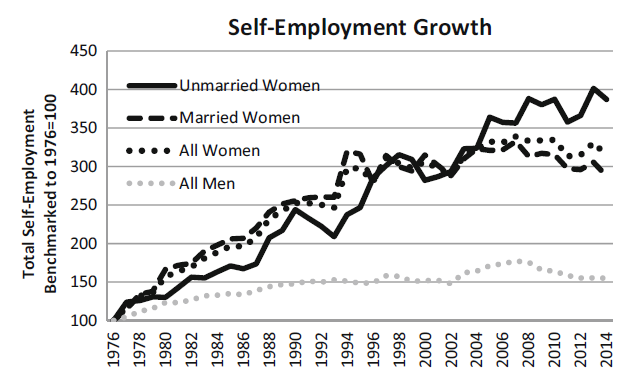
\includegraphics[width=0.75\linewidth]{ch-pastwork/se_growth.PNG}%
    	}%
    \caption{SE Trends in the U.S. Economy (Source: Patrick et al., 2016)} 
\end{figure}

At the U.S. level, recent research advances the idea of different motivations for men and women, with ``more progressive gender attitudes pulling married women from self-employment, while household burdens associated with children pushing them into self-employment as an alternative to not working at all''\footnote{\cite{PatrickStephensWeinstein2016}}. This theory of self-employment as an activity providing married women more resources to balance family and career does not find support in empirical research\footnote{[Wellington, 2006] finds little support that women are increasingly turning to self-employment to balance family and career.}, or the steadily growing share of unmarried women owning a business, observed in Figure 2.1.

\textbf{\textit{Marital status}} is thought to nevertheless affect individual motivations, eliciting different responses to controls. When studies look at data in the aggregate, self-employment is close-to-unanimously positively associated with marital status\footnote{\cite[Page~74]{Parker2004}}. Holding for both business entry and self-employment status, this finding is only weaker in the case of black Americans\footnote{\cite{borjas1986self}} and the English ethnic minority\footnote{\cite{clark2000pushed}}. The general mechanisms thought to explain the positive effect have to do with access to more startup capital in the case of married couples, as well as the availability of labor at below-market rates from the spouse once a business is established\footnote{\cite[Page~75]{Parker2004}}. On top of that, there are associated tax advantages and benefits for the married (healthcare, pension scheme), which can affect the decision to co-enter entrepreneurship\footnote{\cite[Page~75]{BlanchflowerOswald1998}}.

\textbf{\textit{Age}} is often regarded as a proxy for creativity and innovative spirit, one claim being that the older an individual, the less likely to become an entrepreneur. When analyzed in the aggregate, changes in a region's age distribution affect its expected number of startups, the older the population, the lower the share of new businesses\footnote{\cite{Bonte2007}}. In terms of individual patterns, however, the expectation is for most entrepreneurs to be in their 30s and 40s\footnote{\cite{LiangWangLazear2014}}. Work by Quinn (1980)\footnote{\cite{Quinn1980}} tracks labor force participation for older self-employed workers, with results indicating a lower probability to open a business, but also greater chance of maintaining it open. Although most studies address how a region's age distribution influences entrepreneurship rates, or uses an agent's age as a control when testing for other factors, there is growing interest in assessing whether creativity can really be measured via this instrument, and with what results.

The channels through which \textbf{\textit{education}} factors into self-employment are also of great interest to researchers, studies tracking its effect on entry decisions, outcomes, as well as the many other aspects pertaining to running one's business. Higher education and business knowledge are seen as preconditions for ``opening up shop'', yet the expected sign of this coefficient on the probability of becoming self-employed is to be debated. Some authors suggest higher education is a decisive determinant of initial entry into SE, with highly skilled individuals having a higher self-employment rate than other groups in the labor force\footnote{\cite{rees1986empirical}}\hspace{.15em} \footnote{\cite{robinson1994effect}}\hspace{.15em} \footnote{\cite{luber2000growing}}. Yet, when separating boom and bust periods in Finland, Kangasharju and Pekkala (2001)\footnote{\cite{kangasharju2001regional}} find an opposing pattern, with the highly educated being less likely to become self-employed in periods of economic upturn. This finding can be explained by the higher outside demand highly-educated agents experience for their labor, as well as the utility tradeoff associated with entrepreneurship in their case\footnote{\cite{kangasharju2001regional}}. In that sense, running a small firm might not be as attractive as wage work due to ``lower earnings prospects, less stable stream of earnings and the cultural tradition of working in large corporations''\footnote{\cite{kangasharju2001regional}}. In terms of exit rates, the highly educated are also found to have higher exit probability in times of boom, for demand-side reasons similar to those invoked before\footnote{\cite{kangasharju2001regional}}.

Moving beyond years of education and into a discussion of skills more broadly, Lazear (2005)\footnote{\cite{Lazear2005}} introduced the hypothesis that more versatile individuals have higher entrepreneurship rates, with \textbf{\textit{diversified skills}} mattering more than specialized expertise. This has many implications, one being that versatile education, a trait rather difficult to measure with available data, might matter more than higher education in econometric models of entrepreneurship. In terms of entry determinants, versatility as invoked by the author could also be instrumented by a change in industry, if observed to have a significant effect on entrepreneurship decisions. Under this assumption, if entrepreneurial activity is found to be associated with a change in industry, then there's a high degree of adaptability to an individual's skills. The versatility assumption would then paint the picture of entrepreneurs as ``jacks of all trades'' (in Lazear's terminology), able to switch from an industry to the other when starting their own business.

\textbf{\textit{Race}} is an important control for self-employment entry and success patterns, as it speaks to persistent disparities in U.S. business ownership\footnote{ More than 10\% of US workers are self-employed business owners, holding 37.4 percent of total U.S. wealth, yet only 5.1 percent of African American workers and 7.5 percent of Latino workers own businesses compared with more than 11 percent of white and Asian workers (Fairlie and Robb, 2008).}. Having roots in existing racial inequality in education, income, or wealth at the U.S. level, these differences are less understood, with major implications for productivity and economic growth\footnote{\cite{ReynoldsWhite1997}}. The most recent findings place African Americans and Latinos at a lower likelihood to own a business than whites and Asian Americans, and more likely to underperform in running it (lower sales and profits, fewer employees and high closure rates)\footnote{\cite{FairlieRobb2008}}. These patterns speak to the effects of existing disparities, with black-owned businesses starting with substantially less financial capital, and having owners with lower levels of education and business experience on average\footnote{\cite{FairlieRobb2008}}. This extends to exit rates, with higher probabilities to ``close shop'' for Latinos and African Americans\footnote{\cite{FairlieRobb2008}}. At the opposite end, Asian American firms have the strongest performance among racial and ethnic groups after controlling for firm size\footnote{\cite{FairlieRobb2008}}. At the same time, they are more likely to have college educated-owners, an artefact of education patterns at the U.S. level\footnote{\cite{FairlieRobb2008}}.

\textbf{\textit{Immigration status}} is an individual-level variable of key significance, with two opposing views described in literature for its effects on the U.S. economy.
\renewcommand{\labelenumi}{\roman{enumi}}
\begin{enumerate}
  \item Classical economic theory predicts an increases in immigration should decrease employment and price of labor for the native workforce, as it decreases the labor market competitiveness of the later\footnote{\cite{Hanson2012}}. 
  \item Other authors argue that historically, improvements in American living standards have been the consequence of productivity growth, both of capital and labor, a growth resulted from the many innovations in which immigrants often played a key role\footnote{\cite{jones1995culture}}
\end{enumerate}
The body of research on immigration status was incapable of substantiating the belief stemming from classical theory. In turn, high-skilled immigrants are said to make for a growing 25\% of U.S. entrepreneurs, and have equal, if not higher contributions to the production of patents and economic output than natives\footnote{\cite{Kerr2013}}. On average, immigrants also seem to be better trained than natives, when skills are conditioned on educational attainment of comparable levels\footnote{\cite{Kerr2013}}. Although findings attest for the contributions of highly-skilled immigrant entrepreneurs to the U.S. economy, immigration continues to be a divisive issue at the U.S. level, with few, often-blocked policy responses to the consensus in empirical findings\footnote{\cite{Hanson2012}}. 

\textbf{\textit{Availability of capital}} is thought to be a key factor in entrepreneurship decisions, acting as an impediment when not satisfied, as well as an encouraging factor when in abundance. Works by Evans and Leighton (1989)\footnote{\cite{EvansLeighton1989}} or Evans and Jovanovic (1989)\footnote{\cite{EvansJovanovic1989}} find that ceteris paribus, people with greater family assets have a higher probability of switching into self-employment from wage employment. Adding to this, more recent research from Dunn & Holtz-Eakin (2000)\footnote{\cite{DunnHoltzEakin2000}} or Georgellis and Wall (2005)\footnote{\cite{GeorgellisWall2005}} reveals that unexpected gains, such as inheritance or redundancy payments, increase the probability of switching to self-employment. At the other end of the spectrum, capital constraints are the most invoked difficulty by potential entrepreneurs when surveyed about business entry\footnote{\cite{BlanchflowerOswald1998}}. Looking at individual characteristics tracked as far back as childhood personality measurements, Blanchflower and Oswald (1998)\footnote{\cite{BlanchflowerOswald1998}} find no predicting power, and conclude that access to start-up capital remains what matters most for entry decisions. Adding to the access-to-capital framework, Fairlie and Robb (2008)\footnote{\cite{FairlieRobb2008}} find a ``strong positive relationship between startup capital and business outcomes'', firms with higher liquidity levels upon startup being more likely to survive and earn more profit in the long term.

Entrepreneurial activity cannot exist in a vacuum, and often times, business owners are dependent on their partners, on existing social networks and professional ties\footnote{\cite{Lerner2009}}\hspace{.15em}\footnote{\cite[Page~74]{Parker2004}}. \textbf{\textit{Social capital}} matters for business formation, along with existing norms that might inform one's expectations of success\footnote{\cite{Lerner2009}}. Yet, research has been slow to quantify the effects of social capital on entrepreneurship decisions, with most work adopting a sociological perspective of the co-owned business startup. \textit{The Entrepreneurial Group} cites recent surveys denoting that more than half of American business owners hold shared ownership of their startups, going against portrayals of ``the lone visionary'' entrepreneur\footnote{\cite{Ruef2010}}. According to the authors, groups have positive effects on securing credit and advancing initiatives, contributing to higher entry rates\footnote{\cite{Ruef2010}}. Fairlie and Robb (2008)\footnote{\cite{FairlieRobb2008}} complement these findings, denoting that more business experience within a founder's family leads to better outcomes for the enterprise and thus, lower exit probability\footnote{\cite{FairlieRobb2008}}. 


Although some authors claim that urban economics has failed to deliver sufficient work on the spatial aspects of entrepreneurship\footnote{\cite{GlaeserRosenthalStrange2009}}, existing research points to the importance of the \textbf{\textit{local environment}} in the choices of entrepreneurs, as well as subsequent success and influence on the local economy. Self-employment rates vary at the U.S level, with the local business climate and entrepreneurial culture of a region acting as a deterrent or a draw\footnote{\cite{PatrickStephensWeinstein2016}}. Location is often studied in parallel with industry, affecting entrepreneurship decisions via proximity to necessary resources or adherence to economic clusters. One key factor is the concentration of funding sources, the easiest to name being VC investments, with 50\% of total funding going to Silicon Valley and Boston, when these regions only hold 11\% of US population\footnote{\cite{ChatterjiGlaeserKerr2014}}. 

When studying the local determinants of manufacturing startups across cities and industries, Glaeser and Kerr (2008)\footnote{\cite{GlaeserKerr2008}} find that entry is predicted by the presence of local customers, and that new entrants are often drawn to areas with many small suppliers. Ghani et al. (2011)\footnote{\cite{GhaniKerrOConnell2011}} find that the higher the female ownership of local businesses in related industries, the greater the entry rate for new female entrepreneurs, leading to regional spillover effects\footnote{\cite{GhaniKerrOConnell2011}}. This points to the existence of a local entrepreneurship culture, sensible to industry effects and existing gender norms. Adding to this, location variables can also control for uneven natural advantages, or geographic clustering caused by other types of forces, such as the desire to live in NYC, or the location of top research universities\footnote{\cite{ChatterjiGlaeserKerr2014}}. 

\textit{\textbf{Industries}} have evolved, organically or not, to be fairly concentrated in the U.S., attracting business formation via existing opportunities, but also hindering it through persistent entry barriers for particular groups\footnote{\cite{ChatterjiGlaeserKerr2014}}. On the one hand, there are fields that receive significant attention for their innovative characteristics, and that welcome new businesses every year, a prominent example being offered by the tech industry and its growth over the past two decades\footnote{\cite{Berman2014}}. On the other hand, however,  industry segregation by skill level, gender or minority status is still prominent, with a clear lack of diversity across many NAICS subcategories\footnote{\cite{cartwright2011job}}. 

Half a century after the Equal Pay Act of 1963 was passed, women are still found to earn less than men across the board, with industry-specific effects perpetuating these steady trends\footnote{\cite{corbett2012graduating}}\hspace{.15em}\footnote{\cite{cartwright2011job}}. In terms of self-employment participation, the ``disadvantaged worker theory'' denotes that factors hindering general labor market participation might, in fact, encourage workers to start their own business\footnote{\cite{PatrickStephensWeinstein2016}}. The entrepreneurial process would then be seen as both a way to break barriers, as well as an intermediary step toward wage employment\footnote{\cite{PatrickStephensWeinstein2016}}. This theory has nonetheless not echoed in many empirical applications, the convention in literature being to use industry-fixed effects when modeling self-employment status.

The local and national \textbf{\textit{policy environment}} can affect individual entrepreneurship decisions via multiple channels, from helping address liquidity constraints to imposing extra restrictions, from changing corporate taxes to being responsible for the institutional quality and the degree of economic freedom in a given region\footnote{\cite{Williams2013}}. While government loan programs have been found to be generally ineffective in spurring entrepreneurship rates, taxes can have a pronounced effect on the local business climate, being one of the most comprehensively studied factors of innovation policy\footnote{Works include \cite{CullenGordon2006}; \cite{DjankovGanserMcLieshRamalhoShleifer2008}; \cite{Goetz2008}; \cite{Lerner2009}; \cite{Williams2013}.}. To this regard, Djankov et al. (2008)\footnote{\cite{DjankovGanserMcLieshRamalhoShleifer2008}} find that a 10\% increase in the effective corporate tax rate\footnote{ This rate is obtained by dividing a company's total tax bill by its profits.} reduces aggregate investment to GDP ratio by 2 percentage points, and has an adverse impact on entrepreneurial activity. 

Cullen and Gordon (2002)\footnote{\cite{CullenGordon2002}} look at individual incentives, showing that taxes affect the decision to become an entrepreneur due to differences in tax rates on business vs. wage income, as well as the asymmetric tax treatment of losses vs. profits. Using individual tax returns at the U.S. level, their findings reveal that tax law can significantly alter behavior and distort the decision to start a business\footnote{\cite{CullenGordon2002}}. More difficult to measure, institutional quality and the degree of economic freedom also factor into entry and exit decisions, with attempts to quantify the magnitude of their positive effects on self-employment rate\footnote{\cite{Williams2013}}.

Our review of educational attainment and its effects noted that potential founders respond differently to the \textbf{\textit{economic climate}} based on their level of education. In that sense, measures of local economic upturn/downturn affect the opportunity cost of individuals upon switching to self-employment, as well as the expected utility from this activity. Periods of economic boom have negative effects on SE rates for highly-skilled workers, with wage-employment being more advantageous and in greater supply\footnote{\cite{kangasharju2001regional}}. 

In line with the opportunity/necessity distinction in entrepreneurship motivations, \textbf{\textit{unemployment}} can have a positive effect on entry SE rates, with individuals starting a business as an alternative to remaining unemployed\footnote{\cite{Deli2011}}. Research confirms this pattern, finding a positive correlation between local unemployment rates and entry into self-employment for low-ability workers\footnote{\cite{Deli2011}}. These results however, do not hold for high-ability workers, for which there is a negative correlation between unemployment and self-employment\footnote{\cite{Deli2011}}. The interaction between ability and unemployment status is a key component for this type of analysis, speaking to the opportunity cost of highly-skilled workers joining self-employment. 














\chapter{Policy Implications\label{ch:policy}}

\section{The Case for Innovation Policy}

Nascent enterprises on the path to becoming important job creators are of great interest to policymakers. But why is it important for policy to intervene in the equilibrium of births and deaths of companies, and why the focus on the self-employed? Authors that study economic clustering and its effects argue that innovation-oriented policy helps internalize externalities, for at least two reasons: 

\renewcommand{\labelenumi}{\roman{enumi}}
\begin{enumerate}
\item It pays off in the long term to help new firms and incentivize them to remain active, as they will pay taxes for years to come.\footnote{\cite{ChatterjiGlaeserKerr2014}}
\item Spillovers can increase productivity in the aggregate, leading to human capital externalities.\footnote{\cite{Moretti2004}}. 
\end{enumerate}

It is thus justified to foster a culture of innovation and business formation, with hopes for regional development in the long run. There are also redistributive goals to encouraging business formation in specific areas, with measures that serve as example of how to "help poor places instead of poor people"\footnote{\cite{ChatterjiGlaeserKerr2014}}. 

Last but not least, innovation policy can be a means to combat market imperfections, as well as discriminatory factors that might prevent access to funding of specific areas or groups of people\footnote{\cite{ChatterjiGlaeserKerr2014}}. With our findings indicating a persistent gender gap in self-employment, as well as minorities being underrepresented in business ownership, there is legitimacy to policies meant to encourage nascent entrepreneurship in marginalized groups. The idea of an economic and societal cost resulted from marginalizing women in the global economy is not new\footnote{\cite{bakker1994strategic}}\hspace{.15em}\footnote{\cite{blank1993should}}\hspace{.15em}\footnote{\cite{boserup1970women}}, but the  gender integration could become a powerful tool for developing entrepreneurial solutions.  

\section{Findings in Context}

Barriers at the entry stage of the entrepreneurship experience still exist, despite the United States being proclaimed one of the most favorable environments in this respect\footnote{\cite{Autio2007}}. As we saw reflected in our coefficient estimates, women and most minority groups still face significant obstacles to entry. At the same time, men and women respond differently to monetary, lifestyle, policy or economic factors, in ways that might not be incorporated by policy initiatives. In line with this finding, economic literature points out that entry barriers also transfer to the expansion phase for minority-owned businesses, which is costly to productivity at the U.S. level\footnote{\cite{ReynoldsWhite1997}}. 

\subsection{Funding}

As Table A.1 in [Descriptive Statistics] indicates, the Small Business Administration\footnote{The Small Business Administration was created to provide incentives for small businesses at the regional level, in the form of loans, grants and local assistance \cite{SBA}.} has in recent years provided billions of dollars in loans, with values stabilizing around 7 billion a year. We note the persistent gender gap in funding, which could be explained to a great extent by asymmetries in self-employment entry across the two groups, as indicated by our results. Along with that, most funding goes to existing businesses (72\% on average) as opposed to new ones (28\%), and the majority of SBA funds are directed to white-owned firms (over 60\%), which further reflects the distribution of the self-employed. 

With our coefficient estimates indicating a strong positive effect for availability of capital on the likelihood of self-employment, more attention to nascent businesses and their capital constraints from federal organizations such as the SBA could help promote business formation. 

\subsection{Barrier Reduction}

Apart from initiatives meant to provide assistance and funding to nascent small businesses, U.S. cities have in the past implemented policies meant to reduce entry barriers for particular groups, an example being local contracts set aside for businesses owned by women and racial minorities\footnote{\cite{ChatterjiGlaeserKerr2014}}\hspace{.15em}\footnote{\cite{Lerner2009}}. This in turn, is said to have narrowed the black-white self-employment gap in the 80s by more than 3\%\footnote{\cite{ChatterjiGlaeserKerr2014}}.

Given the increasing share of the total population minorities represent in the U.S., policy that targets business formation among these groups will need increasing attention. One can imagine local programs like the 1980s initiatives granting local contracts to women and minority owned businesses getting more traction given that the self-employment gap between men and women, or blacks and whites, does not show signs of decreasing.  

\subsection{Local Supply of Entrepreneurs}

Some policies are meant to increase the so-called "local supply of entrepreneurs", addressing issues of location, education or the availability of information\footnote{\cite{Lerner2009}}. The tendency for the self-employed population "to disproportionately found firms near where one was born" thus challenges policy to ensure the availability of educational programs or science and technology initiatives at the local level, along with ensuring access to basic business knowledge(McAuley, 2013). Adding to this, 42 states currently require entrepreneurial education, more than double from 19 in 2009\footnote{\cite{ChatterjiGlaeserKerr2014}}. 

Given that skill versatility was found to be one of the most important factors in modeling the transition to self-employment, the ability to change industries and market oneself as a "jack of all trades" could be of valuable importance, and more attention must be paid to the degree to which certain regions allows or impede these labor market transitions.

In increasing the supply of local entrepreneurs, high-skilled immigration is also seen as a key issue to be addressed at the federal level. STEM policy is often paired with measures to foster entrepreneurship, and proposals for an entrepreneurial visa providing a path to permanent residency for foreign investors depending on the number of jobs created have been long speculated\footnote{\cite{Dalziel2008}}\hspace{.15em}\footnote{\cite{ChatterjiGlaeserKerr2014}}. However, our findings indicate that there is a negative effect on SE rates of being a high-skilled immigrant in periods of economic upturn, which raises questions about the individual costs and benefits of firm formation for this group.

In evaluating whether if implemented, self-employment policies are effective, it will be crucial in the future to not only understand an agent's motivations for business formation, but also assess self-employment outcomes in terms of jobs created, profits, earnings and so forth. 















\chapter{Data\label{ch:data}}
\chapter{Methodology\label{ch:methods}}


\section {Dependent Variable Discussion}

The current study builds on previous literature and analyzes the factors that motivate or deter men and women to be self-employed. The Kauffman Index of Entrepreneurial Activity is used as an alternative measure for entrepreneurship, along with a comprehensive set of controls from the Current Population Survey, the National Governors' Association,  Angel Capital Association and US Bureau of Economic Analysis\footnote{The events in mind are the dot.com bubble of the early 2000s, along with the Great Recession of 2008.}. The size $N = 9,244,390$ of this constructed dataset makes it nationally representative, and its reach over the 1998-2014 period covering two great shocks on the U.S. economy, makes it temporally comprehensive. By virtue of our data and in line with existing literature, one can compute at least two different econometric models of occupational choice, with dependent variables as delineated in Parker (2004)\footnote{\cite{Parker2004}}: 
\begin{enumerate}
\item The probability of an agent \textit{becoming self-employed} in the second survey month, given individual characteristics, occupational choice and previous work environment, as well as geographic variables and policy indicators.
\item The probability of an agent \textit{being self-employed} at the second survey time, without the condition of wage-employment in the first survey month, with a similar set of controls, minus the ones pertaining to the transition state. 
\end{enumerate}
There are relative merits to these dependent variables, and a comprehensive discussion about their benefits and disadvantages can be found in Parker's theoretical treatment of entrepreneurship decisions\footnote{\cite[Page~26]{Parker2004}}. Several authors argue that (i) is preferable to (ii), as it separates entry and survival effects, a distinction the second model does not accomplish\footnote{\cite{EvansLeighton1989}}. This is due to the fact that the probability of being self-employed at a given time t encompasses the probability of switching into self-employment at a previous time, as well as surviving until time \textit{t}\footnote{\cite{EvansLeighton1989}}. Scholars like Wellington (2001)\footnote{\cite{Wellington2001}} on the other hand, denote that probability (i) excludes people already successfully pursuing self-employment, ignoring an inherently interesting group of observations and making for a small number of new self-employed individuals on a yearly basis. As the goal of the current paper is to estimate what drives entrepreneurship decisions, the first dependent variable, measuring the change from negative to positive self-employment status between two survey times is the most appropriate choice, allowing to capture and explain entrepreneurship as it happens. 


\section{The Probit Method}

We are interested in estimating the probability of an individual switching into self-employment under certain controls and among gender groups. In what follows, we use the Probit method to implement a series of models, with the specification that the Logit  procedure gives rise to similar results, the choice between the two depending largely on individual preference. A Probit model uses the probit link function to model the probability space for a binomial dependent variable\footnote{\cite{AldrichNelson1984}}. We assume there is an unobserved variable of interest, generated by a linear regression model of the form


\begin{dmath}
\mbox{$Y^{*}_{i} = x^{T}_i\beta + u_i = \beta_0 + \beta_1X_{i1} + \beta_2X_{i2} + ... + \beta_kX_{ik} + u_i$}
\end{dmath}
\\
in which:

$Y_i$ is a continuous variable for observation \textit{i}, that is latent or unobservable;

$x^T_i$ is, a row vector of length \textit{k} with regressor values for each observation \textit{i};

$\beta$ is a column vector of length \textit{k} containing the regression coefficients;

$x^T_i\beta$ is a term also known as the index function for observation \textit{i};

$U_i$ is the error term for observation \textit{i}, assumed to follow a normal distribution $N(0, \sigma^2)$. 


The outcomes for the binary choice problem (in our case, whether an individual opens a business or not) are represented by the indicator variable $Y_i$, mapping the unobserved dependent variable $Y^*_i$ as:

\begin{dmath}
\mbox{$Y_i = 1 \mbox{ if } Y^{*}_{i}>0$} \\
\mbox{$Y_i = 0 \mbox{ if } Y^*_i\leq 0$}
\end{dmath}

The indicator variable $Y_i$ represents the observed realizations of the binomial process, with probabilities given by:

\begin{dmath}
\mbox{$Pr(Y_i = 1) = Pr(Y^2_i > 0) = Pr (x^T_i\beta + u_i) >0 $} \\
\mbox{$Pr(Y_i = 0) = Pr(Y^2_i \leq 0) = Pr (x^T_i\beta + u_i) \leq 0 $}
\end{dmath}

Probit models represent binomial probabilities in terms of the standard normal as follows:

\begin{dmath}
\mbox{$Pr(Y_i = 1) = Pr(Y^2_i > 0) = \phi(x^T_i\beta) $} \\
\mbox{$Pr(Y_i = 0) = Pr(Y^2_i \leq 0) = 1 - \phi(x^T_i\beta) $}
\end{dmath}

The probit link function can thus be written as the inverse Gaussian cumulative distribution function, and is estimated using a standard maximum likelihood process\footnote{\cite{AldrichNelson1984}}. In a probit model, the estimate term $X\beta$ corresponds to the z-value of a normal distribution. Higher values of the estimates thus make the event more likely to happen under the given conditions. The data is expected to fit better than in a linear probability estimation, and is guaranteed to lie between 0 and 1. 

\section{Model}

We implement the probit method for three different models of entry probability, one addressing the dataset in the aggregate, and the other two focusing on the female and male samples. The first model (4.6) includes the covariate for gender, while the following two, (4.7) and (4.8) do not.


\begin{dmath}
Y^{*}_{entry} = \beta_0 + \beta_1female + \beta2ed\_years + \beta_3skill\_vers + \beta_4log\_income + \beta_5age + \beta_6age^2 + \beta_7immigr + \beta_8ed*immigr + \beta_9race + \beta_{10}mar\_stat + \beta_{11}hours\_t_0 + \beta_{12}less\_hours\_t_1 + \beta_{13}ind\_t_1 + \beta_{14}gdp\_change + \beta_{15}ed*gdp\_change + \beta_{16}unem + \beta_{17}unem\_rate + \beta_{18}gov\_party + \beta_{19}gov\_change + \beta_{20}region
\end{dmath}


\begin{dmath}
Y^{*}_{entry\_f} = \beta_0 + \beta1ed\_years + \beta_2skill\_vers + \beta_3log\_income + \beta_4age + \beta_5age^2 + \beta_6immigr + \beta_7ed*immigr + \beta_8race + \beta_{9}mar\_stat + \beta_{10}hours\_t_0 + \beta_{11}less\_hours\_t_1 + \beta_{12}ind\_t_1 + \beta_{13}gdp_change + \beta_{14}ed*gdp\_change +\beta_{15}unem + \beta_{16}unem\_rate + \beta_{17}gov\_party + \beta_{18}gov\_change + \beta_{19}region
\end{dmath}

\begin{dmath}
Y^{*}_{entry\_m} = \beta_0 + \beta_1ed\_years + \beta_2skill\_vers + \beta_3log\_income + \beta_4age + \beta_5age^2 + \beta_6immigr + \beta_7ed*immigr + \beta_8race + \beta_{9}mar\_stat + \beta_{10}hours\_t_0 + \beta_{11}less\_hours\_t_1 + \beta_{12}ind\_t_1 + \beta_{13}gdp_change + \beta_{14}ed*gdp\_change + \beta_{15}unem + \beta_{16}unem\_rate + \beta_{17}gov\_party + \beta_{18}gov\_change + \beta_{19}region
\end{dmath}

\section{Clustered Standard Errors}

We suspect observations within the same metropolitan area are correlated, as specific entrepreneurship patterns might exist at this level of granularity. To combat this problem, we implement probit models with clustered standard errors on the metropolitan area variable. A method for modeling error components, clustering maintains the assumption of zero correlation across groups, but allows for within-group correlation. We thus move from the assumption that errors are independent and identically distributed to that of observations within a city being correlated in some way, and their errors clustered.

As a result, Probit estimates remain unbiased, and the cluster-robust error estimator converges to the true standard error as the number of clusters approaches infinity, as opposed to sample size N increasing. In the context of our data, the number of clusters is high enough - we observe over 200 cities, and sufficiently balanced to allow for inference using the cluster-robust estimator. With the same logic, we also implement models with industry clustered standard errors, but choose to report the former. In doing so, we hope to see whether industries have an effect of incentivizing business formation, and whether women can penetrate male-dominated fields via self-employment. 

\section{Sparsity and Perfect Predictions}

The Kauffman Index data gives average annual rates for the transition into self-employment of about 0.5\%. This is comparatively less than the estimates of 10\% of the U.S. population being self-employed at a given time\footnote{\cite{ChatterjiGlaeserKerr2014}}, as our data captures the switch, and not the total number of business owners. This is a legitimate choice for the dependent variable, but one that given the size of our dataset and categorical nature of most explanatory variables, can create a sparsity problem. The presence of sparsity could complicate the implementation of a probit model, with the optimizer reaching a concave region where convergence is not possible. The specification of a ``difficult'' maximization problem beforehand was used to prevent this issue, allowing for the use alternative stepping algorithms in nonconcave regions\footnote{\cite{GouldPitbladoPoi2010}}.

In probit regression, another foreseeable issue is for independent variables, especially when categorical in nature, to perfectly predict one outcome or the other. For our data, industry can become a perfect predictor when used as a categorical variable, with the possibility that for a given \textit{i},

\begin{dmath}
Pr(Y = 0 | Ind_i = 1) = 1
\end{dmath}

This means that the probit coefficient on x must be minus infinity with a corresponding infinite standard error, an improbable estimation. One-way causations of this type were reported and the industry categorical variable \textit{i} eliminated from the regression model\footnote{\cite{GouldPitbladoPoi2010}}. 

\section{Evaluation of Results}

In the Probit model, one unit change in X translates to a $\beta$ change in the z-score of Y\footnote{\cite{AldrichNelson1984}}. In interpreting this result, a positive coefficient on $X_i$ translates to an increase in the predicted probability of $Y_i$. A negative coefficient means the predicted probability of $Y_i$ decreases with an increase in $X_i$\footnote{\cite{AldrichNelson1984}}. Probit p-values show the significance of a parameter, this test statistic following a standard normal distribution. As an equivalent to the coefficient of determination found in OLS regression, Probit computes the McFadden's pseudo R-squared. The total sum of squares is equivalent to the log likelihood of the intercept model, while the residual sum of squares is the log likelihood of the full model. Although caution must be employed in the evaluation of results, this approach is in line with the R-squared as explained variability in OLS, and allows for a comparable interpretation of this statistic\footnote{\cite{Hilbe1996}}\hspace{.2em}\footnote{\cite{Long1997}}. 

\section{Differential effects}

To test whether gender is associated with a difference in the determinants of entrepreneurship entry, we use an F-test of linear restrictions. In this case, we test whether the coefficients for men and women are significantly different from each other in a regression model with interaction terms for being male or female. For each covariate of interest, the null hypothesis is $$H_0 : \beta_{2} - \beta_{1} = 0$$ or, equivalently, $$H_0 : \beta_2 = \beta_1.$$ Knowing the scale of an independent variable affects the size of its coefficient, it is important to note that the regressors corresponding to the coefficients tested are on the same scale. 




\section{Variables and Expectations}

A complete set of controls is provided in Table A.2 [Descriptive Statistics], along with relevant descriptions. The probability of entry is modeled using five categories of covariates that we hypothesize influence an agent's decision to start their own business. 

\begin{figure}[hbtp]
	    \centering{%
		    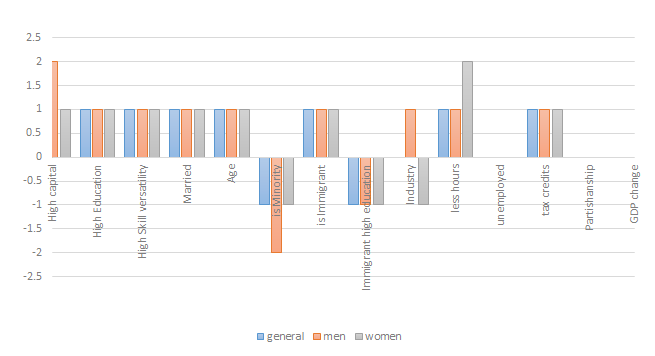
\includegraphics[width=1\linewidth]{ch-methodology/expectations.png}%
       	}%
        \caption{Hypotheses across Covariates of Interest}  
\end{figure}

These are Liquidity constraints, Demographic controls, Job Characteristics, Policy Environment and Location variables. In light of existing literature and with intuitions about where our research can bring further contributions, we frame hypotheses for their effects and underlying mechanisms. Figure 4.1 illustrates our expectations schematically, labeling coefficients by sign and relative magnitude. The scale is for graphing purposes and does not speak to actual estimates.


\subsection{Dependent Variable}

The probability of becoming an entrepreneur $p_{entry}$ is estimated for each individual as the change to self-employment in the second survey month ($t_1$) after conditioned on not being self-employed in the first one ($t_0$). The sample mean is around 0.5\%, with a slight decrease in the yearly average for the period after 2008. 



\subsection{Individual-level variables}

\textbf{Liquidity Constraints.} Availability of capital ($log\_income$) is measured as the natural logarithm of an individual's family income at survey time $t_0$. Higher levels of liquidity are expected to lead to a higher likelihood of self-employment $p_{entry}$, and we are interested in how this effect varies across genders. We expect positive coefficients for both men and women, and given literature, suspect men to be more responsive to family income. 

\textbf{Education.} Educational attainment ($ed\_years$) is measured in years of schooling for both men and women. We expect this variable to have a strong positive influence on self-employment entry, as higher levels of human capital often mean better access to resources needed to start one's business. 

\textbf{Skill versatility.} We compute versatility ($skill\_vers$) as a binary for whether the respondent changed industry in the given year, instrumented on educational attainment. Given the literature, a higher degree of skill versatility should lead to positive effects on the self-employment rate, with differences to be analyzed across genders. If women experience more rigid labor markets, and might pursue less marketable courses of study at the same level of educational attainment, they would have less possibilities for industry change. As a result, we expect to observe a coefficient that is smaller in magnitude in their case. 

\textbf{Marriage.}  Marital status ($i.marstat$) is a categorical variable, with the differentiated labels:
\begin{enumerate}
\singlespacing
\item Married, spouse present
\item Married, spouse in armed forces
\item Married, spouse absent
\item Widowed
\item Divorced
\item Never married
\end{enumerate}

Household characteristics are expected to play a large role in one's motivations to start a business, with literature predicting both genders being positively incentivized by being married. 

\textbf{Marriage and Finances.} We compute an interaction term $mar\_income$ to test whether marriage status influences the way people value financial stability in their choice to open a business. For this purpose, a binary for marriage was created, aggregating the six categories to only two values. If marriage is indeed a positive influence on the motivation to start a business, then this interaction should have a positive effect, denoting that the more liquidity couples dispose of, the greater their likelihood of business formation. 

\textbf{Age.} We expect age to be a push factor for entry decisions, with a threshold suspected for positive effects. We fit a quadratic term for the coefficients on age, and expect to see an upside down parabola with different degrees of steepness for men and women [Figure 4.2]. According to this hypothesis, individuals are more likely to become self-employed as they are becoming older and getting closer to a certain age, after which the curve slopes downward. If confirmed by coefficient estimates, this finding could nuance the discussion of aggregate age effects. 

\begin{figure}[hbtp]
	  \centering{%
		  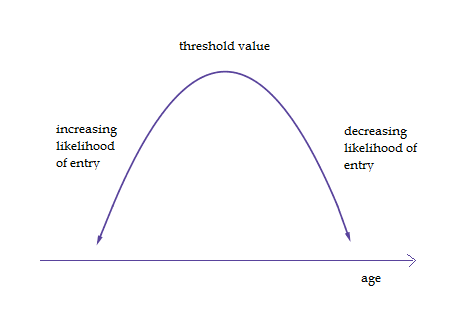
\includegraphics[width=0.6\linewidth]{ch-methodology/concavedown.png}%
    	}%
    \caption{Schematic Representation of Expected Age Effects} 
\end{figure}

\textbf{Race.} Membership to a minority group ($i.race$) is computed as a categorical variable, with coefficients indicating whether deterrents exist for particular groups. We expect being Black or Hispanic to present negative estimates for the effect on self-employment, with coefficients smaller in magnitude for the female sample. This is predicted due to more barriers associated with being a man in these racial groups. The coefficient on being Asian is expected to produce a positive effect on the self-employment rate, with interest in whether there is a differential on gender. 


\textbf{Immigration.} Immigrant status ($immigr$) is computed as a binary, with consensus in literature for positive self-employment outcomes within this category. It is nonetheless important to differentiate effects according to education, and we add an interaction term on skill level for both genders. The expectation is of a negative effect of highly-skilled immigrant status on the wish to start a business, as respondents in this group are more likely to experience a higher demand on their skills and a regulatory environment less favorable for risk taking. We are interested in whether this effect holds to the same degree for both genders, with a case to be made for different motivations for female/male immigrants. 


\subsection{Employment Characteristics}

\textbf{Industry.} We record industry at survey time $t_0$ and $t_1$, with granularity for sub-sectors coded according to NAICS guidelines. Agriculture, mining and construction were dropped from the sample, our research being interested in self-employment initiatives in manufacturing and the services sector. We use categorical variables for major industries of interest, with an interest in observing whether women see self-employment as a way to break barriers in traditionally male-dominated fields (e.g. engineering, software development or financial services).

Women are known to be underrepresented at the senior management level of companies, which only deters progress in the efforts for full gender integration\footnote{\cite{olivetti2016dp11034}}. These gaps are said to originate from ``a limited pipeline of women in entry- and mid-level roles'', which is all the more prominent in male-heavy fields\footnote{\cite{adams2012beyond}}. As a result, we wonder whether self-employment can address this issue, allowing women to break into industries by starting their own companies. If coefficients for certain industries are positive and significant for this group at survey time $t_1$, data might point to a certain barrier-breaking mechanism associated with starting one's own business. 


\textbf{Hours worked.} The $hours \geq 0$ worked by an agent at his main job are recorded at both survey times, with a binary variable for less hours following the transition from $se\_t_0 = 0$ to $se\_t_1 = 1$. We first test whether the hours worked at survey time $t_0$, conditioned $hours\_t_0 \geq 0$, contribute to the motivation to become self-employed. We are also interested whether starting a business is positively motivated by a greater degree of flexibility at work, as expressed by the coefficient on $less_hours$. 

Workers could turn to self-employment because of its associated non-monetary benefits, and not necessarily for the economic incentives. To test whether the positive effect is controlled by marriage status, we implement an interaction term for working less at $t_1$ and being married. In that sense, some married women might be more likely to adopt self-employment for the benefit of a more flexible schedule if household characteristics point to it. 

\textbf{Unemployed.} Unemployment status at $t_0$ ($unem$) becomes a measure of necessity entrepreneurship, with a positive coefficient expected for respondents who were out of work at the first survey time. The extent to which being unemployed matters for men and women has proven ambiguous, and in our research we wish to asses whether the coefficient differs in magnitude across the two groups.


\subsection{Policy Environment}

\textbf{Tax incentives.} Tax credits are measured by a binary ($tax\_credit$) indicating the existence of a tax break on new business investment in the respondent's state in the given year\footnote{The author is aware that the research framework could also use the actual corporate tax rate in a state and during the given year, a popular approach to measuring the friendliness of a policy environment to new businesses. However, the intent is to capture as much of the heterogeneity in states' different treatment of new businesses as possible, and the availability of tax credits is an approach that could provide new insights}. We are interested in how these credits incentivize business formation, and whether asymmetric effects exist for men and women. We hypothesize the coefficient is positive, and that it might vary across groups.

\textbf{Local governance.} The partisanship of the current governor ($rep\_gov$, $dem\_gov$ and $indep\_gov$) is added to asses whether men and women respond differently to political factors in deciding to pursue self-employment at a given time. Particular types of economic policies - small business loans, the willingness to implement tax breaks, programs that engage women and minorities, etc - might be more closely associated with a political ideology than the other, and could affect the incentives of people wanting to open a business. 

At the same time, a binary for party change in state level governance ($gov\_change$) has been computed, testing whether partisanship shifts provide cues for new programs and incentives. If this is the case, a positive coefficient might indicate there are new motivations associated with a change in political landscape, and there is an interest to assess whether men and women take such cues differently. 


\subsection{Macroeconomic Conditions}

\textbf{State GDP.} The coefficient on state GDP change ($gdp\_change$) from the past year measures the extent to which an individual's likelihood to start a business might respond to periods of economic upturn or downturn. This effect is complex, encompassing both a sense of real economic conditions affecting one's labor market prospects, as well as the degree to which they are assimilated by respondents into the decision to start a business.

\textbf{Education and Economic Performance.} We compute an interaction term of education and local economic prospects ($ed\_econ$), hoping to provide an intuition for an agent's demand for wage labor at a given time. As such, a negative coefficient on this interaction term would indicate that in times of economic upturn, high skill is rewarded more by wage employment. In times of downturn, there might be more incentives to join self-employment. The extent to which this effect varies for men and women speaks to both individual incentives, as well as how the U.S. labor market values work and skill level across genders. 

\textbf{State Unemployment.} The state unemployment rate ($unem\_rate$) is measure for the current year, the previous year and the change between periods. We expect a negative coefficient on unemployment, as periods of economic downturn fail to provide the necessary incentives for individuals to take the risks associated with business formation. Differences in gender might be due to different manifestations of risk aversion, as well as labor prospects in times of high unemployment. \\

We cluster errors on \textbf{metropolitan area}, and use states as controls that speak to the spatial concentration of business formation. Given that location data is categorical in nature, we expect certain states to be more influential than others, with those overlapping with historically innovative regions such as Silicon Valley or Route 128 to result in positive coefficients, while others negatively contributing to entry probability. When used to model entry rates, these variables might also capture up-and-coming entrepreneurship hubs, as opposed to established innovation clusters. 

































\chapter{Results\label{ch:results}}

Table B.1 shows estimates for models (4.6), (4.7) and (4.8) implemented via the probit specification. Significant coefficients for demographic variables, economic conditions, as well as industry effects were reported for different levels of $\alpha$. The total probit model estimates a negative coefficient $\beta_{female} = -0.204$, statistically significant at the $\alpha = 1\%$ level and among the biggest in magnitude across covariates. This proves the need to investigate how the probability to enter entrepreneurship differs for men and women, and what factors matter for each group.

\section{Demographic variables}

\begin{figure}[hbtp]
	  \centering{%
		  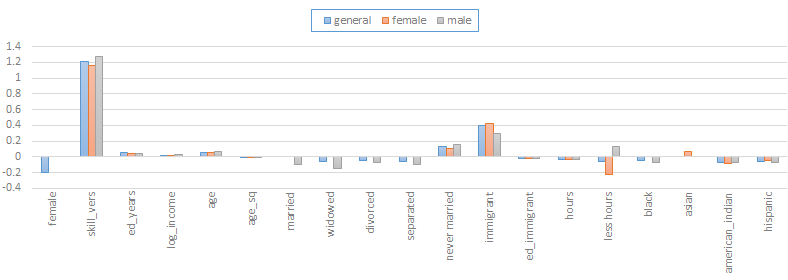
\includegraphics[width=1\linewidth]{ch-results/individual.png}%
    	}%
    \caption{Magnitude of Significant Coefficients for Individual Level Variables} 
\end{figure}

Figure 5.1 illustrates the magnitude of significant coefficients comparatively across the three models for variabes that pertain to the agent-level. We note that for covariates like skill diversification or immigrant status, the three estimates are fairly consistent in magnitude and sign, while variables like $less\_hours$, the number of hours associated with the transition to self-employment, have differential effects on men and women. 

\subsection{Education}

Educational attainment is one of the most significant demographic factors to affect entry decisions, with a positive coefficient $\beta_{ed} = 0.0497$ for the entire dataset, a similar value for women, $\beta_{ed} = 0.0482$ and a smaller effect for men, $\beta_{ed} = 0.0418$. The F statistic testing the equality of the coefficients shows a significant difference across genders, with a greater magnitude for the effect of female educational attainment. 

The interaction term for skill level and immigration status also provides important insights as to how education affects entrepreneurship decisions. While immigrant status is positively associated with likelihood of self-employment entry, with $\beta_{immigr} = 0.427}$ for women and $\beta_{immigr} = 0.291$ for men, this control has negative effects when interacted with years of education. In this case, the overall coefficient is $\beta_{ed*immigr} = - 0.0240$, with a stronger negative effect for women ($\beta_{ed*immigr} = - 0.0254$) than for men ($\beta_{ed*immigr} = - 0.0163$). 

Education also factors in when interacted with GDP change at the state level, causing differential effects for periods of economic upturn and downturn.  Here, men record a negative coefficient $\beta_{ed*econ} = -0.00126$, meaning that in times of economic upturn (positive GDP change), a higher number education years makes it less probable for them to start a business. For women, this hypothesis does not hold, with the interaction between education and GDP change having a positive coefficient $\beta_{ed*econ} = 0.00142$. For periods of economic upturn, higher education for this group translates to a higher probability for business entry. 

\subsection{Skill Versatility}

An arguably related measure, an individual's skill versatility has a significant positive effect on the likelihood of self-employment, with the greatest magnitude among the covariates in Figure 5.1. To this regard, the coefficients are $\beta_{change} = 1.165$ for women and $\beta_{change} = 1.271$ for men, indicating a greater degree of flexibility leads to a higher probability of self-employment. The estimates are not significantly different across genders, and are in line with the results for the general sample, pointing to a robust effect of this factor on self-employment entry. 

\subsection{Age}

The coefficients on age describe a quadratic function with $\alpha <0 $, given $\beta_{age} = 0.0578$ and $\beta_{age^2} = -0.000534$ for the complete dataset. For women, these values are similar, with $\beta_{age} = 0.0578$ and $\beta_{age^2} = -0.000534$, while for men they are greater in magnitude, with $\beta_{age} = 0.0629$ and $\beta_{age^2} = -0.000595$. The shape of the concave-down parabola implies a positive effect of age on self-employment until a maximum value is reached. For any value greater than this vertex, there is a negative effect of age on the probability of entry. These results are consistent for the data in the aggregate, as well as when differentiated by gender.

\subsection{Immigrant Status}

Immigrant status on its own also affects the probability of entry, with positive coefficients across all three groups. When not interacted with educational attainment, $\beta_{immigr} = 0.404$ for all data, with an estimate similar for women -- $\beta_{immigr} = 0.427$ and significantly lower for men -- $\beta_{immigr} = 0.291$. This gender difference is significant, as reported by our F test. When conditioned on years of education, the coefficient changes sign and magnitude, as we previously saw. 

\subsection{Marriage Status}

Marriage status was analyzed both on its own and in interaction with other factors. Being married was found to have a significant negative effect on men's self-employment entry, with $\beta_{married} = -0.954$. The effect on women is of opposing sign, with $\beta_{married} = 0.0259$ denoting a positive influence on the likelihood of transitioning into self-employment. At the other end, the coefficients on not having been married contradict previous research, with positive effects on the probability of starting a business across all groups ($\beta_{never\_married} = 0.112$ for women and $\beta_{never\_married} = 0.156$ for men). Here, gender differences are not observed, with equally positive effects on the probability of starting a business. When marriage status is instrumented with income or hours worked, we find no significance to the new coefficients, disproving the extent to which being married can affect monetary motivations or induce different work patterns for men and women.

\subsection{Race}

Race affects the probability of entry, with most minority groups having negative coefficient estimates for both genders. Being American Indian has the greatest negative effect on the probability of self-employment for the whole dataset, followed by being Hispanic and Black. Being Asian is here the only covariate with a positive effect on entry probability ($\beta_{asian} = 0.0439$). Differences in magnitude still exist between men and women, with black males having a significantly more negative coefficient than females ($\beta_{black\_male} = -0.0726$ versus $\beta_{black\_female} = -0.0196$), a pattern that holds for hispanics as well ($\beta_{hisp\_male} = -0.0755$ versus $\beta_{black\_female} = -0.0470$). At the other end, being an Asian woman has a greater positive coefficient than the male counterpart, with coefficient estimates $\beta_{asian\_female} = 0.0675$ and $\beta_{asian\_male} = 0.0083$ respectively. 

\section{Capital constraints}

In terms of the availability of capital, the level of family income at the first survey time is found to have a significant positive effect on the probability of self-employment, with a bigger coefficient for men ($\beta_{income} = 0.0260$) than women ($\beta_{income} = 0.0157$). This difference is significant when subjected to an F-test, and speaks to the important effect of capital in incentivizing business formation.

\section{Employment Characteristics}

Past employment characteristics are a telling covariate, with negative coefficients on hours worked at $t_0$ across groups. The estimates are $\beta_{hours} = -0.0377$ for women and $\beta_{hours} = -0.03893$, values that are not significantly different at the $\alpha = 1 \%$ level. The more an individual works at their current job, the less likely the transition into self-employment is, a finding that holds across genders.

Lifestyle changes vary in their power to incentivize business formation among men and women. The coefficient measuring the difference in hours between survey times denotes that among men, self-employment is positively affected by the promise of less hours worked ($\beta_{less\_hours} = 0.128$). For women, this is not the case, with $\beta_{less\_hours} = 0.128$. The prospect of working less has a negative impact on women's decision about business entry, a significantly different effect from their male counterparts. Contrary to expectations, the signs for these coefficients are not altered by marriage status, with no statistical significance for the associated interaction term. 

\begin{figure}[hbtp]
	  \centering{%
		  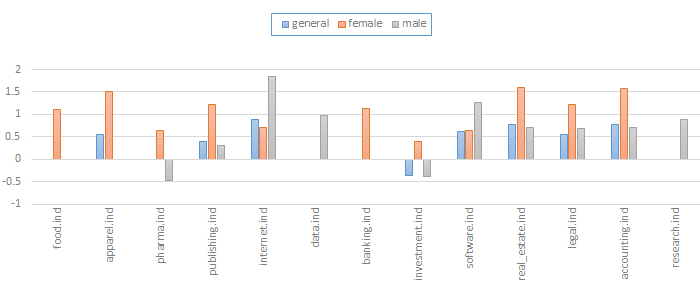
\includegraphics[width=1\linewidth]{ch-results/industry.png}%
    	}%
    \caption{Magnitude of Significant Industry Coefficients by Gender} 
\end{figure}

As illustrated by Figure 5.2, results also show consistent patterns of gender division across industries, with fields more traditionally occupied by men remaining prominent choices for new businesses for this group. The coefficients for men in tech industries are $\beta_{Data} = 0.967$, $\beta_{Software} = 1.259$ or $\beta_{Internet} = 0.967$. All the while, female self-employment is more positively incentivized by industries traditionally avoided by men, as indicated by $\beta_{Apparel} = 0.967$ or $\beta_{Accounting} = 1.575$ for the female sample.

It is important to note that both the male-dominated and female-dominated industries generate coefficients on men/women respectively that significantly surpass the values for the general sample [see Figure 5.2]. In that sense, the probit model for the data in the aggregate estimates an average effect of certain industries on probability of self-employment entry, one that misses the important asymmetries across genders. 

\section{Environment Variables}

\begin{figure}[hbtp]
	  \centering{%
		  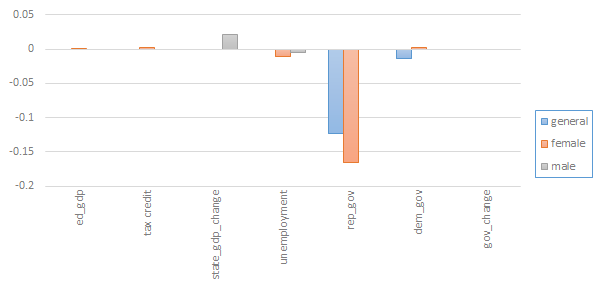
\includegraphics[width=1\linewidth]{ch-results/external.png}%
    	}%
    \caption{Magnitude of Significant Coefficients for Environment Variables} 
\end{figure}

Figure 5.3 plots significant coefficients for the external factors thought to affect an agent's decision to enter self-employment. Here, we note more pronounced effects of the gender split, with most covariates affecting men or women significantly, but not both groups. 

\subsection{Economic Conditions}

Unemployment is a significant indicator of how local economic conditions affect self-employment rates, with negative coefficients $\beta_{unemployment} = -0.0113$ for women and $\beta_{unemployment} = -0.00514$ for men. Although of the same sign, these values are found to differ in magnitude at the $\alpha = 1\% $ significance level, women being less likely to start a business when there is a high unemployment rate in their respective state. 

\subsection{Policy Climate}
Tax incentives for starting a business also show more significant responsiveness in the sample of female respondents, with  $\beta_{tax\_credit} = 0.0021$. For men, this coefficient is negative, $\beta_{tax\_credit} = -0.0131$, pointing to a reverse effect of tax credit on business formation. Instead of contributing to the likelihood of business formation, tax credits are estimated to have a negative effect for the male sample. This difference is significant at at the $\alpha = 1\% $ level. 

The party affiliation of state governors is found to matter differently across gender groups. Having a republican governor has a significant negative effect on business formation for women, with $\beta_{rep\_gov} = -0.165$, while having a democratic governor seems to have a slight positive effect on women's self-employment, with  $\beta_{dem\_gov} = 0.0017$. For the male sample, the effects are of opposite sign ($\beta_{rep\_gov} = 0.0775$ and $\beta_{rep\_gov} = -0.0103$), but not significant at the $\alpha = 5\% $ level. 

\section{Evaluation of Results}

The majority of reported coefficients are significant at the $\alpha = 5\% $ level, with some particular patterns for men and women. For covariates like being married or widowed, the effect seems to only be significant for men, while the interaction between GDP change and education level or local governance indicators hold more in the case of women. For the general model, $PseudoR^2 = 0.542$ for the general model, and similar values for men - $PseudoR^2 = 0.5328$ and women - $PseudoR^2 = 0.5595$. Although we are able to explain the highest degree of variability for the female sample, overall the regression models provide a good fit.
























\chapter{Discussion\label{ch:disc}}

As expected, gender is a significant determinant in the general model for entrepreneurship, as seen in the first column of Table B.1. The most important other factors for this model are education, income, immigrant status, skill versatility, minority group, marriage status and industry-specific effects. While some determinants abide by our formulated hypotheses in the probit coefficients they produce (income, age, skill versatility), others provide significantly different results than those anticipated (marital status, immigrant status). Results for all significant covariates across the three samples can be visualized in Figure B.1 [Regression Results]. In comparing the general model with the gendered-differentiated ones, we note the standard empirical approach to investigating the determinants of business entry ignores important asymmetries between men and women's responsiveness to policy, macroeconomic conditions or individual characteristics that might lead to business formation. 

\section{Availability of Capital}
Our findings highlight that women are positively, but to a lesser degree than men motivated by capital upon starting a business. This might speak to a certain degree of risk aversion observed in women more than in men\footnote{\cite{adams2012beyond} observe that women do not take as many risks at the workplace as men do, in an attempt to avoid being perceived poorly by colleagues. This behavioral pattern disappears when authors look at female CFO's, indicating that arriving at this leadership position allows women to suppress perception concerns. In turn, female CFO's are observed to be just as, and often times even more risk-taking than their male counterparts.}, which can echo in investment decisions and allocation of current income. If women are less risk-taking in the aggregate, then they might not perceive monetary surplus as a chance to start their own company, and think instead in longer-term frameworks. Our finding then suggests that from a policy standpoint, infusions of liquidity might not have immediate effects in spurring female entrepreneurship. 

\section{Education and Skills}
We predicted higher education would lessen incentives for immigrant men and women to start companies, as an indicator of the demand for their wage-labor at a given time. The effect on business formation was indeed negative, but smaller in magnitude for immigrant women than for men. One explanation is that women in immigrant groups might still encounter less demand for their wage labor than their male counterparts, despite having similar levels of educational attainment\footnote{\cite{ReynoldsWhite1997}}. If their work is not rewarded to a similar extent for highly educated immigrant women to prefer wage employment to opening a business, this adds to the observation that the U.S. labor market doesn't offer equal opportunities across genders.

Regarding the mixed effects of education, we hypothesized that in times of economic upturn, highly educated agents will be less likely to start a business for similar demand-side reasons as those invoked above. While this effect was found to be negative in the aggregate, education was less likely to deter self-employment in periods of economic upturn in the case of women. This finding could suggest labor market discrimination, but might also substantiate the risk-aversion theory in making women less likely to respond immediately to changes in economic conditions.

Our results provide direct empirical evidence that skill versatility matters to a greater extent than the level of education, a claim speculated in theoretical frameworks for entrepreneurship\footnote{\cite{Lazear2005}}, but not fully analyzed in empirical research. This robust finding holds across genders, with the ability to change industries having positive effects on the probability of self-employment. 

\section{Marriage}

We found that marital status does not produce the positive effects suggested across self-employment literature, with most positive coefficients observed for those who have never been married. The theory of supportive spouses\footnote{ Referring to the idea that married couples are more likely to open businesses due to more access to capital, as well as the option to work for the new company at below-market rates.}, tax benefits and below-market price labor could still hold, but the incentives for single people to start businesses are equally, if not more prominent. While the view of the risk taking, lone entrepreneur might find some backing in these results, a more realistic interpretation relies on the power of professional networks, friend groups and support that goes beyond one's life partner in facilitating business ventures. 

\section{Minority Group}

The coefficients across minority groups indirectly reveal the significant extent to which African-Americans, Hispanics or American-Indians are held back in the U.S. labor market when it comes to starting a business. In that sense, the negative estimates confirmed our expectations, with the only group experiencing positive effects on entrepreneurship entry being Asian Americans. Across the minority groups for which business formation is less likely, women were observed to experience a slightly smaller negative effect. An explanation might consist of a smaller degree of stigma associated with women in these groups when compared to their male counterparts\footnote{\cite{AlbaRumbautMarotz2005}}, which could translate to less expected barriers in accessing funding and resources. 

\section{Lifestyle Choices}
Lifestyle choices motivating entrepreneurship also differ for men and women, with men being more likely to switch to self-employment if it implies less hours worked, while women experience the reverse. This adds nuance to assumptions in existing literature, which denote women might choose self-employment for the flexibility benefits and ability to work less\footnote{\cite{bertrand2013gender}}. Marital status is not able to substantiate this claim, suggesting there is more to the story of some married women opening a business to have more time for household work. To that end, women might regard self-employment as a leadership opportunity and as a response to barriers in advancement encountered in wage-employment\footnote{\cite{olivetti2016dp11034}}. Therefore, they invest time and effort into running their own company, and demonstrate a high time commitment throughout. Men might not develop similar incentives, viewing self-employment as a transitioning state, or as an activity providing a more flexible lifestyle. It is important to note our data targets individuals in metropolitan and non-metropolitan areas across the U.S., which can differ in terms of gender attitudes. 


\section{Industry Effects}

Industries remain similarly segregated as in the case of wage employment, with women not being able to penetrate traditionally male-dominated fields by the act of opening a business. Software engineering, data processing or internet services attract men to a significantly greater degree than the sample average, while industries like apparel, real estate or accounting tend to motivate female presence [illustrated in Figure 6.1 below]. Although women are just as likely to change industry upon joining self-employment as men, there are still differences in the fields they choose. 

This finding could be partially explained by differences in field of study across genders, with women underrepresented in science and technology subjects at similar level of educational attainment\footnote{\cite{olivetti2016dp11034}}. It could also mean certain barriers in wage employment\footnote{Some examples include less representation, barriers to entry, barriers to advancement, wage discrimination.} get transferred to self-employment, and that opening one's business describes an unrealistic mechanism for surpassing existing frictions. 

\begin{figure}[hbtp]
	  \centering{%
		  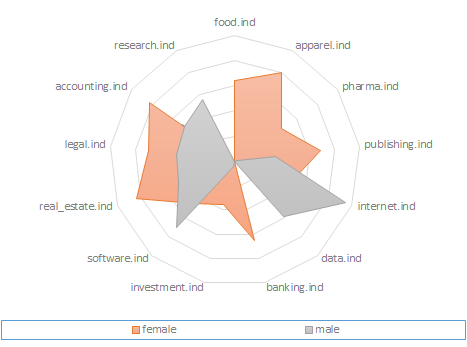
\includegraphics[width=0.7\linewidth]{ch-discussion/industry_fm.png}%
    	}%
    \caption{Magnitude of Positive Industry Coefficients by Gender} 
\end{figure}

\section{Economic Conditions}

In terms of environment variables, men were found to be more responsive to macroeconomic conditions, while women tend to be motivated to a greater degree by tax credits. The first finding might speak to how genders perceive changes in local economies\footnote{Research on this topic is not comprehensive, but some insights are provided by Leach et al. (1999)\footnote{\cite{LeachHayhoeTurner1999}}, who look at how female and male college students perceive their own economic well-being differently, with differential effects across factors. Difference in behaviors that originate in perceived economic well-being have also been studied, some examples being credit card use (Armstrong & Craven, 1993) or spending habits (Hayhoe et al., 2000).}, but also the degree to which they are allowed to flexibly adapt to them. If women's degree of labor mobility is more limited, awareness of periods of economic boom might not automatically translate to better opportunities in wage employment and less motivation to start a business. 

On the tax side, women's responsiveness to these types of policies might indicate their efficiency in targeting prospective female business owners, but also a different outlook for this particular group. Specifically, responsiveness to tax credits might point to a long-term focus in planning and more responsibility as household providers/caretakers/shoppers/expense managers in the case of women. In this light, men's responsiveness to current economic conditions would indicate a more short-term approach, with planning to cover current business indicators. 

\section{Political Climate}
Our findings regarding political climate highlight that women tend to be motivated to start a business if they have a democratic governor, and experience negative effects from republican local governance. One assumption underlying this result might have to do with policies attributed to both parties, and their differential appeal to female voters. It might be that democratic measures encourage a better business climate for women, with policies targeting work-life balance that have no effect on men's considerations. 

Similarly, although the Republican party is associated with tax breaks and a friendlier regulatory regime, small businesses haven't historically been the center of republican measures, with bigger companies thought to stand at the core of republican policies\footnote{\cite{Brown2010}}. Since new businesses often start small, this can influence women's perception of the business climate in their given state if associated with Republican governance. If an agent's sense of worth and perception of risk are \textit{gendered qualities}\footnote{Here, we refer to different perceptions of risk and self-worth explored by psychological work.}\footnote{\cite{adams2012beyond}}, this would further explain why men would not be affected by this policy focus, and why it makes a significant negative difference for women.

Nonetheless, we find no significance to partisanship \textit{changes} at the local level, which could point to an alternative interpretation of the results. If the leadership climate is merely a reflection of the voter base, then states that are historically republican-governed might correspond to different attitudes about policy, business ownership and gender roles. The partisanship of the governor can thus be an instrument that measures gender attitudes at the local level, attitudes that affect the number of women that might pursue entrepreneurship at a given time. This is in line with the lack of statistical significance for partisanship change at the local level, pointing that transitions in governance might not matter as much as the general ideology of a region.

\section{Robustness Check}

\subsection{External Validity}

Our models were able to capture a significant proportion of the variability in self-employment entry, with Pseudo $R^2$ coefficients surpassing 0.5. There are however, areas that could benefit from further exploration, a more comprehensive set of variables being expected to add to the current research in insightful ways. 

In terms of education and its effect on self-employment rates, it is known that in most OECD countries men and women reach similar attainment levels\footnote{\cite{charles2002equal}}. However, there is a persistent gender gap in \textit{educational choices} across genders, with women being a majority in fields like health and education, and underrepresented in more technical programs, like hard sciences and engineering\footnote{\cite{charles2002equal}}. Given that our data doesn't capture field of study, but only level of educational attainment and industry of choice, one can suspect that similar education level might not bring the same effects across individuals, especially since technical fields are more often associated with both entrepreneurship of innovation, as well as persistent gender gaps. 

Entrepreneurship is often associated with \textit{``greater flexibility in terms of an agent's discretion over the length, location and scheduling of their work time''}\footnote{\cite{Quinn1980}}. It is thus expected for people with poor health or disabilities to have a higher probability of self-employment, as a way to avoid workplace discrimination\footnote{\cite{Quinn1980}}. The relation between self-employment and ill-health or disability could be an important control for self-employment decisions, one to be explored with more generous data. Research\footnote{ Works by \cite{BurkeFitzroyNolan2002}; \cite{GeorgellisWall2005} or \cite{CowlingTaylor2001} do not treat the number of children an agent has as the covariate of interest, but use it as a control.} also finds that children act as a greater impediment on a female's entrepreneurial career than that of a male, a factor our model does not control for due to data limitations. In the future, the role of children on parents' decisions to become entrepreneurs, as well as quit self-employment could be studied to capture whether changes of societal perceptions on parenthood have occurred, or whether traditional parenting patterns are still in place.  















\chapter{Conclusion\label{ch:conclusion}}

The current paper models the determinants of entrepreneurship entry decisions at the U.S. level, asking whether and how men and women respond differently to factors of interest. We expand on existing literature addressing gender asymmetries in self-employment, individual attributes and their effect on entry rates, as well as work on local environments and their role in fostering entrepreneurship. The probability of an agent becoming an entrepreneur is estimated via a probit model, as a function of socio-economic factors, demographic controls, local business climate, liquidity constraints and occupational choice. For every model, errors are clustered by metropolitan area, and coefficient equality is tested across gender groups.

When considering men and women's self-employment choices in the United States from 1998 to 2014, we find variation on a number of important dimensions in their motivations to start a business. At the individual level, availability of capital remains an important positive factor, along with skill versatility and educational attainment. Minority status and being married are significant deterrents, with similar effects for men and women. The differences occur when looking at prefered lifestyle choices, with female self-employment being associated with more hours worked and male self-employment, with a smaller time commitment. 

With regards to external factors, we find women are incentivized to a greater extent by tax credits and the state of the political climate, while men respond to positive changes in the local economy. We relate this finding to behavioral science literature highlighting different perceptions of risk and decision making under uncertainty for men and women\footnote{\cite{adams2012beyond}\cite{koellinger2013gender}}, and encourage future research in this respect. Across industries, we find a pattern of female underrepresentation in STEM fields, similar to the one in wage-employment, which disproves the hypothesis of a breaking-barriers mechanism to starting one's business. 

The need to understand and adapt to the changing demographics of the United States\footnote{One of the most recent projections of the U.S. Census Bureau for the future U.S. population denotes that "by 2044, more than half of all Americans are projected to belong to a minority group (any group other than non-Hispanic White alone); and by 2060, nearly one in five of the nation's total population is projected to be foreign born. + cite Colby, S. and Ortman, J.M. (2015)} and that of gender integration in the labor market are topics closely related to the goal of maintaining competitiveness on the global scale. To that end, the United States economy might not be able to afford productivity deterrents and unexploited growth sources due to persistent barriers for women and minorities. In conclusion, our work suggests that both empirically and theoretically, the factors affecting women's employment choices, particularly those of starting a business should become a priority that informs better-targeted policies. 
\appendix % all chapters following will be labeled as appendices
\chapter{Descriptive Statistics\label{ch:stats}}
% Please add the following required packages to your document preamble:
% \usepackage{booktabs}
\begin{table}[htb]
\centering
\footnotesize
\caption{SBA Lending Statistics}
\label{my-label}
\begin{tabular}{@{}lllllllllll@{}}
\toprule
\multicolumn{1}{c}{} & \multicolumn{1}{c}{2011} & \multicolumn{1}{c}{} & \multicolumn{1}{c}{2012} & \multicolumn{1}{c}{} & \multicolumn{1}{c}{2013} & \multicolumn{1}{c}{} & \multicolumn{1}{c}{2014} & \multicolumn{1}{c}{} & \multicolumn{1}{c}{2015} &  \\ \midrule
\textit{\textbf{All}} & \$10B & \multicolumn{1}{c}{} & \$4,7B &  & \$5.84B &  & \$5.73B &  & \$7.26B &  \\
White & \$6.6B & 66\% & \$3B & 65\% & \$3.6B & 62\% & \$3.2B & 56\% & \$4.21B & 58\% \\
AllMinority & \$2,6B & 26\% & \$1.2B & 25\% & \$1.54M & 26\% & \$1.64B & 29\% & \$2.06B & 28\% \\
Am\_Indian & \$45M & 0\% & \$23M & 0\% & \$27.1M & 0\% & \$23.5M & 0\% & \$42.2M & 1\% \\
Asian & \$1.96B & 20\% & \$860M & 18\% & \$1.15B & 20\% & \$1.23B & 21\% & \$1.47B & 20\% \\
Black & \$178M & 2\% & \$75M & 2\% & \$98M & 2\% & \$111M & 2\% & \$131M & 2\% \\
Hispanic & \$380M & 4\% & \$220M & 5\% & \$270M & 5\% & \$275M & 5\% & \$413M & 6\% \\
Other & \$892M & 9\% & \$460M & 10\% & \$700M & 11\% & \$891M & 16\% & \$989M & 14\% \\
\textit{\textbf{Gender}} &  &  &  &  &  &  &  &  &  &  \\
Female Owned & \$1.54B & 15\% & \$786M & 17\% & \$915M & 16\% & \$9423M & 16\% & \$1.16B & 16\% \\
(50\% or less) & & & & & & & & & & & 
Female Owned& \$1.17B & 12\% & \$603M & 13\% & \$760M & 13\% & \$700M & 12\% & \$928M & 13\% \\
(more than 50\%) & & & & & & & & & & & 
Male Owned & \$7.33B & 73\% & \$3.33B & 71\% & \$4.16B & 71\% & \$4.1B & 71\% & \$5.17B & 71\% \\
ExistingBusiness & \$7.65B & 76\% & \$3.44B & 73\% & \$4.34B & 74\% & \$4.2B & 72\% & \$4.86B & 67\% \\
NewBusiness & \$2.33B & 23\% & \$1.27B & 27\% & \$1.49B & 26\% & \$1.59B & 28\% & \$2.38B & 33\% \\
Rural & \$2.29B & 23\% & \$801M & 17\% & \$839M & 14\% & \$946M & 17\% & \$1.22B & 17\% \\
Urban & \$7.76B & 77\% & \$3.91B & 83\% & \$5B & 86\% & \$4.78B & 83\% & \$6B & 83\% \\ \bottomrule
\multicolumn{11}{l}{\footnotesize M = millions of U.S. dollars; B = billions of U.S. dollars}\\
\multicolumn{11}{l}{\footnotesize Source: Small Business Administration}\\
\end{tabular}
\end{table}

\chapter{Regression Results\label{ch:appendix}}
\tablespacing
\small
\begin{longtable}{p{3 cm} p{2.25 cm} p{2.25 cm} p{2.25 cm}}
\caption{Entry Probability with Metropolitan Area-Clustered SE}
\centering
\hline\hline
            &\multicolumn{1}{c}{(1)}&\multicolumn{1}{c}{(2)}&\multicolumn{1}{c}{(3)}\\
            &\multicolumn{1}{c}{entry}&\multicolumn{1}{c}{entry}&\multicolumn{1}{c}{entry}\\
            &\multicolumn{1}{c}{(total)}&\multicolumn{1}{c}{(female)}&\multicolumn{1}{c}{(male)}\\
\hline
female      &      -0.204\sym{***}&                     &                     \\
            &    (-22.39)         &                     &                     \\
ed\_years    &      0.0497\sym{***}&      0.0482\sym{***}&      0.0418\sym{***}\\
            &     (21.91)         &     (13.60)         &     (14.71)         \\

log\_income  &      0.0169\sym{**} &      0.0157\sym{*}  &      0.0260\sym{***}\\
            &      (2.75)         &      (2.03)         &      (3.43)         \\

age         &      0.0578\sym{***}&      0.0568\sym{***}&      0.0629\sym{***}\\
            &     (31.10)         &     (20.98)         &     (18.24)         \\

age\_sq      &   -0.000534\sym{***}&   -0.000521\sym{***}&   -0.000595\sym{***}\\
            &    (-25.60)         &    (-16.97)         &    (-15.38)         \\
immigr      &       0.404\sym{***}&       0.427\sym{***}&       0.291\sym{***}\\
            &      (6.73)         &      (4.25)         &      (5.52)         \\
ed\_immigr   &     -0.0240\sym{***}&     -0.0254\sym{***}&     -0.0163\sym{***}\\
            &     (-6.01)         &     (-3.80)         &     (-4.38)         \\
ed\_econ     &  -0.0000134         &     0.00142\sym{*}  &    -0.00126         \\
            &     (-0.03)         &      (2.30)         &     (-1.95)         \\

hours       &     -0.0379\sym{***}&     -0.0377\sym{***}&     -0.0389\sym{***}\\
            &    (-69.48)         &    (-74.49)         &    (-49.03)         \\

less\_hours  &     -0.0534\sym{***}&      -0.226\sym{***}&       0.128\sym{***}\\
            &     (-3.38)         &     (-9.50)         &      (8.97)         \\

hisp        &     -0.0595\sym{***}&     -0.0470\sym{**} &     -0.0755\sym{**} \\
            &     (-3.69)         &     (-2.63)         &     (-3.27)         \\
tax\_credit  &    -0.00512         &     0.00209         &     -0.0131         \\
            &     (-0.24)         &      (0.10)         &     (-0.46)         \\
ind\_change  &       1.217\sym{***}&       1.165\sym{***}&       1.271\sym{***}\\
            &    (125.81)         &     (87.88)         &     (92.98)         \\
state\_gdp\_change&     0.00411         &     -0.0150         &      0.0209\sym{*}  \\
            &      (0.60)         &     (-1.65)         &      (2.15)         \\
rep\_gov     &      -0.123\sym{*}  &      -0.165\sym{**} &     -0.0775         \\
            &     (-2.16)         &     (-2.66)         &     (-1.31)         \\
dem\_gov     &      -0.140\sym{*}  &      -0.172\sym{**} &      -0.103         \\
            &     (-2.51)         &     (-2.94)         &     (-1.73)         \\
gov\_change  &    -0.00778         &     -0.0231         &      0.0100         \\
            &     (-0.48)         &     (-1.25)         &      (0.54)         \\
Food.ind &      0.0889         &       1.099\sym{***}&      -0.240         \\
            &      (0.54)         &      (5.70)         &     (-1.15)         \\
Textile.ind &       0.159         &       1.300\sym{**} &      -0.327         \\
            &      (0.46)         &      (3.16)         &     (-0.83)         \\
Apparel.ind &       0.559\sym{***}&       1.505\sym{***}&    -0.00929         \\
            &      (3.46)         &      (8.57)         &     (-0.03)         \\
Printing.ind &       0.393\sym{**} &       1.351\sym{***}&       0.160         \\
            &      (3.13)         &     (10.14)         &      (1.17)         \\
Pharma.ind &      -0.289         &       0.634\sym{**} &      -0.466\sym{*}  \\
            &     (-1.53)         &      (3.06)         &     (-1.96)         \\
Publishing.ind &       0.398\sym{**} &       1.215\sym{***}&       0.316\sym{*}  \\
            &      (3.09)         &      (7.30)         &      (2.15)         \\
Internet.ind &       0.884\sym{***}&       .699\sym{***}&       1.852\sym{***}\\
            &      (6.80)         &      (3.39)         &      (9.83)         \\
Data.ind &       0.120         &   0.0109     &       0.967\sym{***}       \\
            &      (0.70)         &      (0.05)         &        (3.96)       \\
Banking.ind &       0.217         &       1.131\sym{***}&      0.0442         \\
            &      (1.15)         &      (3.67)         &      (0.16)         \\
Investment.ind &      -0.368\sym{**} &       0.396\sym{**} &      -0.391\sym{**} \\
            &     (-2.78)         &      (2.86)         &     (-2.62)         \\
Software.ind &       0.628\sym{***}&      0.639\sym{***} &       1.259\sym{***}\\
            &      (5.42)         &     (5.28)         &             (10.23)  \\
Real\_Estate.ind &       0.784\sym{***}&       1.596\sym{***}&       0.700\sym{***}\\
            &      (6.55)         &     (12.51)         &      (5.69)         \\
Legal.ind &       0.559\sym{***}&       1.229\sym{***}&       0.677\sym{***}\\
            &      (4.70)         &     (10.00)         &      (5.66)         \\

Accounting.ind &       0.770\sym{***}&       1.575\sym{***}&       0.713\sym{***}\\
            &      (6.60)         &     (11.80)         &      (5.49)         \\
Research.ind\_t1 &      0.0103         &      -0.113 &      0.891\sym{***}         \\
            &      (0.08)         &      (-0.85)        &      (6.29)        \\
Black      &     -0.0456\sym{*}  &     -0.0196         &     -0.0726\sym{**} \\
            &     (-2.55)         &     (-0.87)         &     (-2.97)         \\
Asian      &      0.0439         &      0.0675\sym{*}  &     0.00829         \\
            &      (1.39)         &      (1.98)         &      (0.18)         \\
Native\_American      &     -0.0724\sym{**} &     -0.0811\sym{**} &     -0.0716\sym{*}  \\
            &     (-2.79)         &     (-2.74)         &     (-2.10)         \\
South    &      0.0803\sym{**} &       0.103\sym{***}&      0.0499         \\
            &      (2.79)         &      (3.46)         &      (1.52)         \\

West    &       0.136\sym{***}&       0.179\sym{***}&      0.0882\sym{**} \\
            &      (5.46)         &      (6.60)         &      (3.15)         \\
2002.year   &     -0.0386\sym{*}  &     -0.0428         &     -0.0302         \\
            &     (-2.37)         &     (-1.66)         &     (-1.34)         \\
2005.year   &     -0.0428\sym{*}  &     -0.0363         &     -0.0457         \\
            &     (-2.04)         &     (-1.20)         &     (-1.71)         \\
Married   &     -0.0347         &      0.0259         &     -0.0954\sym{**} \\
            &     (-0.99)         &      (0.50)         &     (-2.59)         \\
Widowed   &     -0.0639\sym{*}  &     -0.0493         &      -0.142\sym{**} \\
            &     (-2.51)         &     (-1.67)         &     (-3.11)         \\
Divorced   &     -0.0413\sym{***}&     -0.0219         &     -0.0723\sym{***}\\
            &     (-3.63)         &     (-1.47)         &     (-5.08)         \\
Separated  &     -0.0551\sym{*}  &     -0.0411         &     -0.0904\sym{*}  \\
            &     (-2.49)         &     (-1.74)         &     (-2.41)         \\
Never\_Married   &      0.133\sym{***}&      0.112\sym{***}&      0.156\sym{***}\\
            &     (8.17)         &     (4.96)         &     (9.59)         \\

\_cons      &      -3.987\sym{***}&      -4.932\sym{***}&      -3.980\sym{***}\\
            &    (-24.36)         &    (-27.59)         &    (-22.04)         \\
\hline
\(N\)       &     5214221         &     2774014         &     2414844         \\
\(Pseudo R^2\)       &   0.5420         &    0.5595       &    0.5328      \\
\hline\hline
\multicolumn{4}{l}{\footnotesize \textit{.ind} denotes the industry at $t_0$, when subject was SE}\\
\multicolumn{4}{l}{\footnotesize \textit{t} statistics in parentheses}\\
\multicolumn{4}{l}{\footnotesize \sym{*} \(p<0.05\), \sym{**} \(p<0.01\), \sym{***} \(p<0.001\)}\\
\end{longtable}




% Make the bibliography single spaced
\singlespacing

% add the Bibliography to the Table of Contents
\cleardoublepage
\ifdefined\phantomsection
  \phantomsection  % makes hyperref recognize this section properly for pdf link
\else
\fi
\addcontentsline{toc}{chapter}{Bibliography}

\section{Test Section—Citation Examples}
This document is an example of BibTeX using in bibliography management. Three items are cited: \textit{The \LaTeX\ Companion} book \cite{LeoniFalk2010}, the Einstein journal paper \cite{BEA}, and the Donald Knuth's website \cite{AcsArmington2006}. The \LaTeX\ related items are \cite{RodrguezFierroGarridoNavarro2015,Kerr2010}. 

% include your .bib file
\bibliographystyle{unsrt}
\bibliography{thesis}

%Bibliographic references


\end{document}

